\newpage
\appendix
\section{Models}
We select in total 37 models for evaluation and analysis. Our results in the main text only include aligned models (GPT-4, Gemini-1.5, and 15 open-source models). Besides the aligned models, we also evaluate 7 open-source base models using~\ruler. We use the performance of Llama2-7b (base) and Llama2-7b (chat) at context length of 4K as the threshold for determining effective context size. 
In our analysis section, we evaluate in total 11 models, including model series Yi and LWM, as well as models of novel architectures, including Mamba and RWKV. 

\label{models}
\begin{table}[H]
\centering
\resizebox{0.99\linewidth}{!}{
\begin{tabular}{@{}lcccl@{}}
\toprule
Model & Aligned & Size & Context Length & Huggingface~\citep{huggingface} / API \\
\midrule
GPT-4~\citep{openai2023gpt4} & \ding{51} & - & 128K & \texttt{gpt-4-1106-preview} \\
Gemini-1.5~\citep{gemini} & \ding{51} & - & 1M & \texttt{gemini-1.5-pro} \\
\midrule
Llama3.1~\citep{llama3-1} & \ding{51} & 70B & 128K & meta-llama/Meta-Llama-3.1-70B-Instruct \\
Llama3.1~\citep{llama3-1} & \ding{51} & 8B & 128K & meta-llama/Meta-Llama-3.1-8B-Instruct \\
Command-R-plus~\citep{command-r} & \ding{51} & 104B & 128K & CohereForAI/c4ai-command-r-plus \\
% Command-R~\citep{command-r} & \ding{51} & 35B & 128K & CohereForAI/c4ai-command-r-v01 \\
Qwen2~\citep{qwen2} & \ding{51} & 72B & 128K & Qwen/Qwen2-72B-Instruct \\
% Qwen1.5~\citep{qwen} & \ding{51} & 72B & 128K & Qwen/Qwen1.5-72B-Instruct \\
Yi~\citep{yi} & \ding{51} & 34B & 200K & 01-ai/Yi-34B-200K \\
Mixtral-8x22B~\citep{mixtral} & \ding{51} & 39B/141B & 32K & mistralai/Mixtral-8x22B-Instruct-v0.1 \\
% Mixtral-8x7B~\citep{mixtral} & \ding{51} & 12.9B/46.7B & 32K & mistralai/Mixtral-8x7B-Instruct-v0.1 \\
Mistral-v0.2~\citep{misral7bv2} & \ding{51} & 7B & 32K & mistralai/Mistral-7B-Instruct-v0.2 \\
GLM4~\citep{glm4} & \ding{51} & 9B & 1M & THUDM/glm-4-9b-chat-1m \\
% GLM3~\citep{glm} & \ding{51} & 6B & 128M & THUDM/chatglm3-6b-128k \\
GradientAI/Llama3~\citep{llama3}  & \ding{51} & 70B & 1M & gradientai/Llama-3-70B-Instruct-Gradient-1048k \\
% GradientAI/Llama3~\citep{llama3}  & \ding{51} & 8B & 1M & gradientai/Llama-3-8B-Instruct-Gradient-1048k \\
Phi3-medium~\citep{phi3} & \ding{51} & 14B & 128K & microsoft/Phi-3-medium-128k-instruct \\
% Phi3-mini~\citep{phi3} & \ding{51} & 3.8B & 128K & microsoft/Phi-3-mini-128k-instruct \\
LWM~\citep{lwm} & \ding{51} & 7B & 1M & LargeWorldModel/LWM-Text-Chat-1M \\
DBRX~\citep{dbrx} & \ding{51} & 36B/132B & 1M & databricks/dbrx-instruct \\
Together~\citep{together-instruct} & \ding{51} & 7B & 32K & togethercomputer/Llama-2-7B-32K-Instruct \\
LongChat~\citep{longchat} & \ding{51} & 7B & 32K & lmsys/longchat-7b-v1.5-32k \\
LongAlpaca~\citep{longlora} & \ding{51} & 13B & 32K & Yukang/LongAlpaca-13B \\
\midrule
Mixtral-base~\citep{mixtral} & \ding{55} & 8x7B & 32K & mistralai/Mixtral-8x7B-v0.1 \\
Mistral-base~\citep{misral7bv2} & \ding{55} & 7B & 32K & alpindale/Mistral-7B-v0.2-hf \\
LWM-base~\citep{lwm} & \ding{55}  & 7B & 1M & LargeWorldModel/LWM-Text-1M \\
LongLoRA-base~\citep{longlora} & \ding{55}  & 7B & 100K & Yukang/Llama-2-7b-longlora-100k-ft \\
Yarn-base\citep{yarn} & \ding{55}  & 7B & 128K & NousResearch/Yarn-Llama-2-7b-128k \\
Together-base~\citep{together} & \ding{55}  & 7B & 32K & togethercomputer/Llama-2-7B-32K \\
Jamba-base~\citep{jamba} & \ding{55} & 52B & 256K & ai21labs/Jamba-v0.1 \\

\midrule

Llama2 (chat)~\citep{llama2} & \ding{51} & 7B & 4K & meta-llama/Llama-2-7b-chat-hf \\
Llama2 (base)~\citep{llama2} & \ding{55}  & 7B & 4K & meta-llama/Llama-2-7b-hf \\
\midrule
Yi series~\citep{yi} & \ding{51} & 6B,9B & 200K & 01-ai/Yi-(6B,9B)-200K \\
LWM series~\citep{lwm} & \ding{51} & 7B & 128K,256K,512K & LargeWorldModel/LWM-Text-Chat-(128K,256K,512K) \\
LWM-base series~\citep{lwm} & \ding{55}  & 7B  & 32K,128K,256K,512K & LargeWorldModel/LWM-Text-(32K,128K,256K,512K) \\
Mamba~\citep{mamba} & \ding{55} & 2.8B & 2K & state-spaces/mamba-2.8b-slimpj \\
RWKV~\citep{rwkv} & \ding{55} & 7B & 4K & RWKV/v5-Eagle-7B-HF \\

\bottomrule
\end{tabular}}
\caption{Information of evaluated and analyzed models in~\ruler.}
\end{table}



\clearpage
\section{Task Configurations}
\label{task_configurations}
\ruler~is designed to be configurable to allow for diverse sequence lengths and task complexities. For each task, there arises combinatorially large number of configurations one can adopt. In the main text, we evaluate the models with 13 representative tasks spanning the four categories of \ruler. Our task selection process is described in the next appendix section.
% Since our tasks have flexible configurations to setup different complexities, we select total 13 tasks in \ruler. 
\begin{itemize}[leftmargin=*]
    \item \textbf{Retrieval}: In S-NIAH, we include the passkey retrieval~\citep{landmark} and the vanilla NIAH~\citep{needle}, both use word-number as key-value and differ only by the background haystack. Additionally, we change the value type to UUID, for the purpose of testing model robustness at retrieving long strings from context. For MK-NIAH, we add three distractor needles into the haystack. We also include existing setups from previous works: line retrieval~\citep{longchat} and key-value retrieval~\citep{lostmiddle} with the haystack filled entirely with distractor needles. 
For MV-NIAH and MQ-NIAH, we test 4 values and queries respectively. 
    \item \textbf{Multi-hop tracing}: For VT, we insert 1 chain with 4 name-binding hops, totally 5 variable names need to be returned. 
    \item \textbf{Aggregation}: For CWE, in total 10 common words need to be returned, each appears 30 times whereas the uncommon words appear 3 times each.
For FWE, we set $\alpha$ to 2.0 in Zeta distribution for sampling synthetic words. 
    \item \textbf{QA}: For QA, we augment SQuAD~\citep{squad} and HotpotQA~\citep{hotpotqa} to simulate long-context scenario. They are representative of single-hop and multi-hop question answering tasks respectively.
\end{itemize}
% For S-NIAH, we use the well-known passkey retrieval~\citep{landmark} and vanilla NIAH~\citep{needle} as the baseline. 
% Additionally, we change the value type with UUID to test the robustness of retrieving a long sequence. 
% For MK-NIAH, we add three extra needle keys into haystack as initial test as well as the line retrieval~\citep{longchat} and key-value retrieval~\citep{lostmiddle} with haystack filled with all distracted needles. 
% For MV-NIAH and MQ-NIAH, we test 4 values and queries respectively. 


\begin{table}[H]
\centering
\small
\resizebox{\linewidth}{!}{
\begin{tabular}{c|p{0.26\linewidth}|p{0.26\linewidth}|p{0.26\linewidth}}
\toprule
\multirow{2}{*}{\textbf{Task}} & 
\multicolumn{3}{c}{\textbf{Configurations}} \\
\cmidrule{2-4}
 & 
\multicolumn{1}{c|}{\textbf{Subtask-1}} & 
\multicolumn{1}{c|}{\textbf{Subtask-2}} & 
\multicolumn{1}{c}{\textbf{Subtask-3}} \\
\midrule
\begin{tabular}[t]{@{}l@{}}Single\\NIAH\end{tabular} & 
\begin{tabular}{@{}l@{}}type\_key = word\\type\_value = number\\type\_haystack = repeat\\\textbf{$\sim$passkey retrieval}\end{tabular} &
\begin{tabular}{@{}l@{}}type\_key = word\\type\_value = number\\type\_haystack = essay\\\textbf{$\sim$vanilla NIAH}\end{tabular} & 
\begin{tabular}{@{}l@{}}type\_key = word\\type\_value = uuid\\type\_haystack = essay\\ \  \end{tabular}
\\
\midrule
MK-NIAH & 
\begin{tabular}{@{}l@{}}num\_keys = 4\\type\_key = word\\type\_value = number\\type\_haystack = essay\end{tabular} &
\begin{tabular}{@{}l@{}}num\_keys = full haystack\\type\_key = word\\type\_value = number\\\textbf{$\sim$line retrieval}\end{tabular} &
\begin{tabular}{@{}l@{}}num\_keys = full haystack\\type\_key = uuid\\type\_value = uuid\\\textbf{$\sim$KV retrieval}\end{tabular}
\\
\midrule
MV-NIAH & 
\multicolumn{3}{l}{num\_values = 4, type\_key = word, type\_value = number, type\_haystack = essay}
\\
\midrule
MQ-NIAH & 
\multicolumn{3}{l}{num\_queries = 4, type\_key = word, type\_value = number, type\_haystack = essay}
\\
\midrule
VT & 
\multicolumn{3}{l}{num\_chains = 1, num\_hops = 4}
\\
\midrule
CWE & 
\multicolumn{3}{l}{freq\_cw = 30, freq\_ucw = 3, num\_cw = 10}
\\
\midrule
FWE & 
\multicolumn{3}{l}{$\alpha$ = 2.0}
\\
\midrule
QA & 
dataset = SQuAD & 
\multicolumn{2}{l}{dataset = HotpotQA}
\\
\bottomrule
\end{tabular}}
\caption{Our total 13 task configurations in \ruler.}
\label{tab:benchmark-task}
\end{table}

\clearpage
\section{Task Correlation Analysis}
\label{task_correlation}
 \ruler~is designed under the assumption that tasks across different categories are able to reveal distinct model behaviors. We conduct a preliminary correlational study to confirm the validity of task categories and guide the selection of representative tasks. We evaluate eight open-sourced models at various context sizes across 18 task configurations. Each task can then be represented with a vector of model performance at various context sizes. The 18 task vectors are then clustered via agglomorative clustering algorithm, using correlation coefficient as the distance metric.
 As shown in Figure~\ref{fig:corr_heatmap}, while certain tasks exhibit moderate correlations with others, tasks in each of the four categories (NIAH, VT, AG, QA) form cohesive clusters of their own without redundancy. We further eliminate a few tasks that correlate highly with other tasks within the same cluster, and finalize 13 tasks for later large scale evaluation.
\begin{figure*}[h]
    \centering
    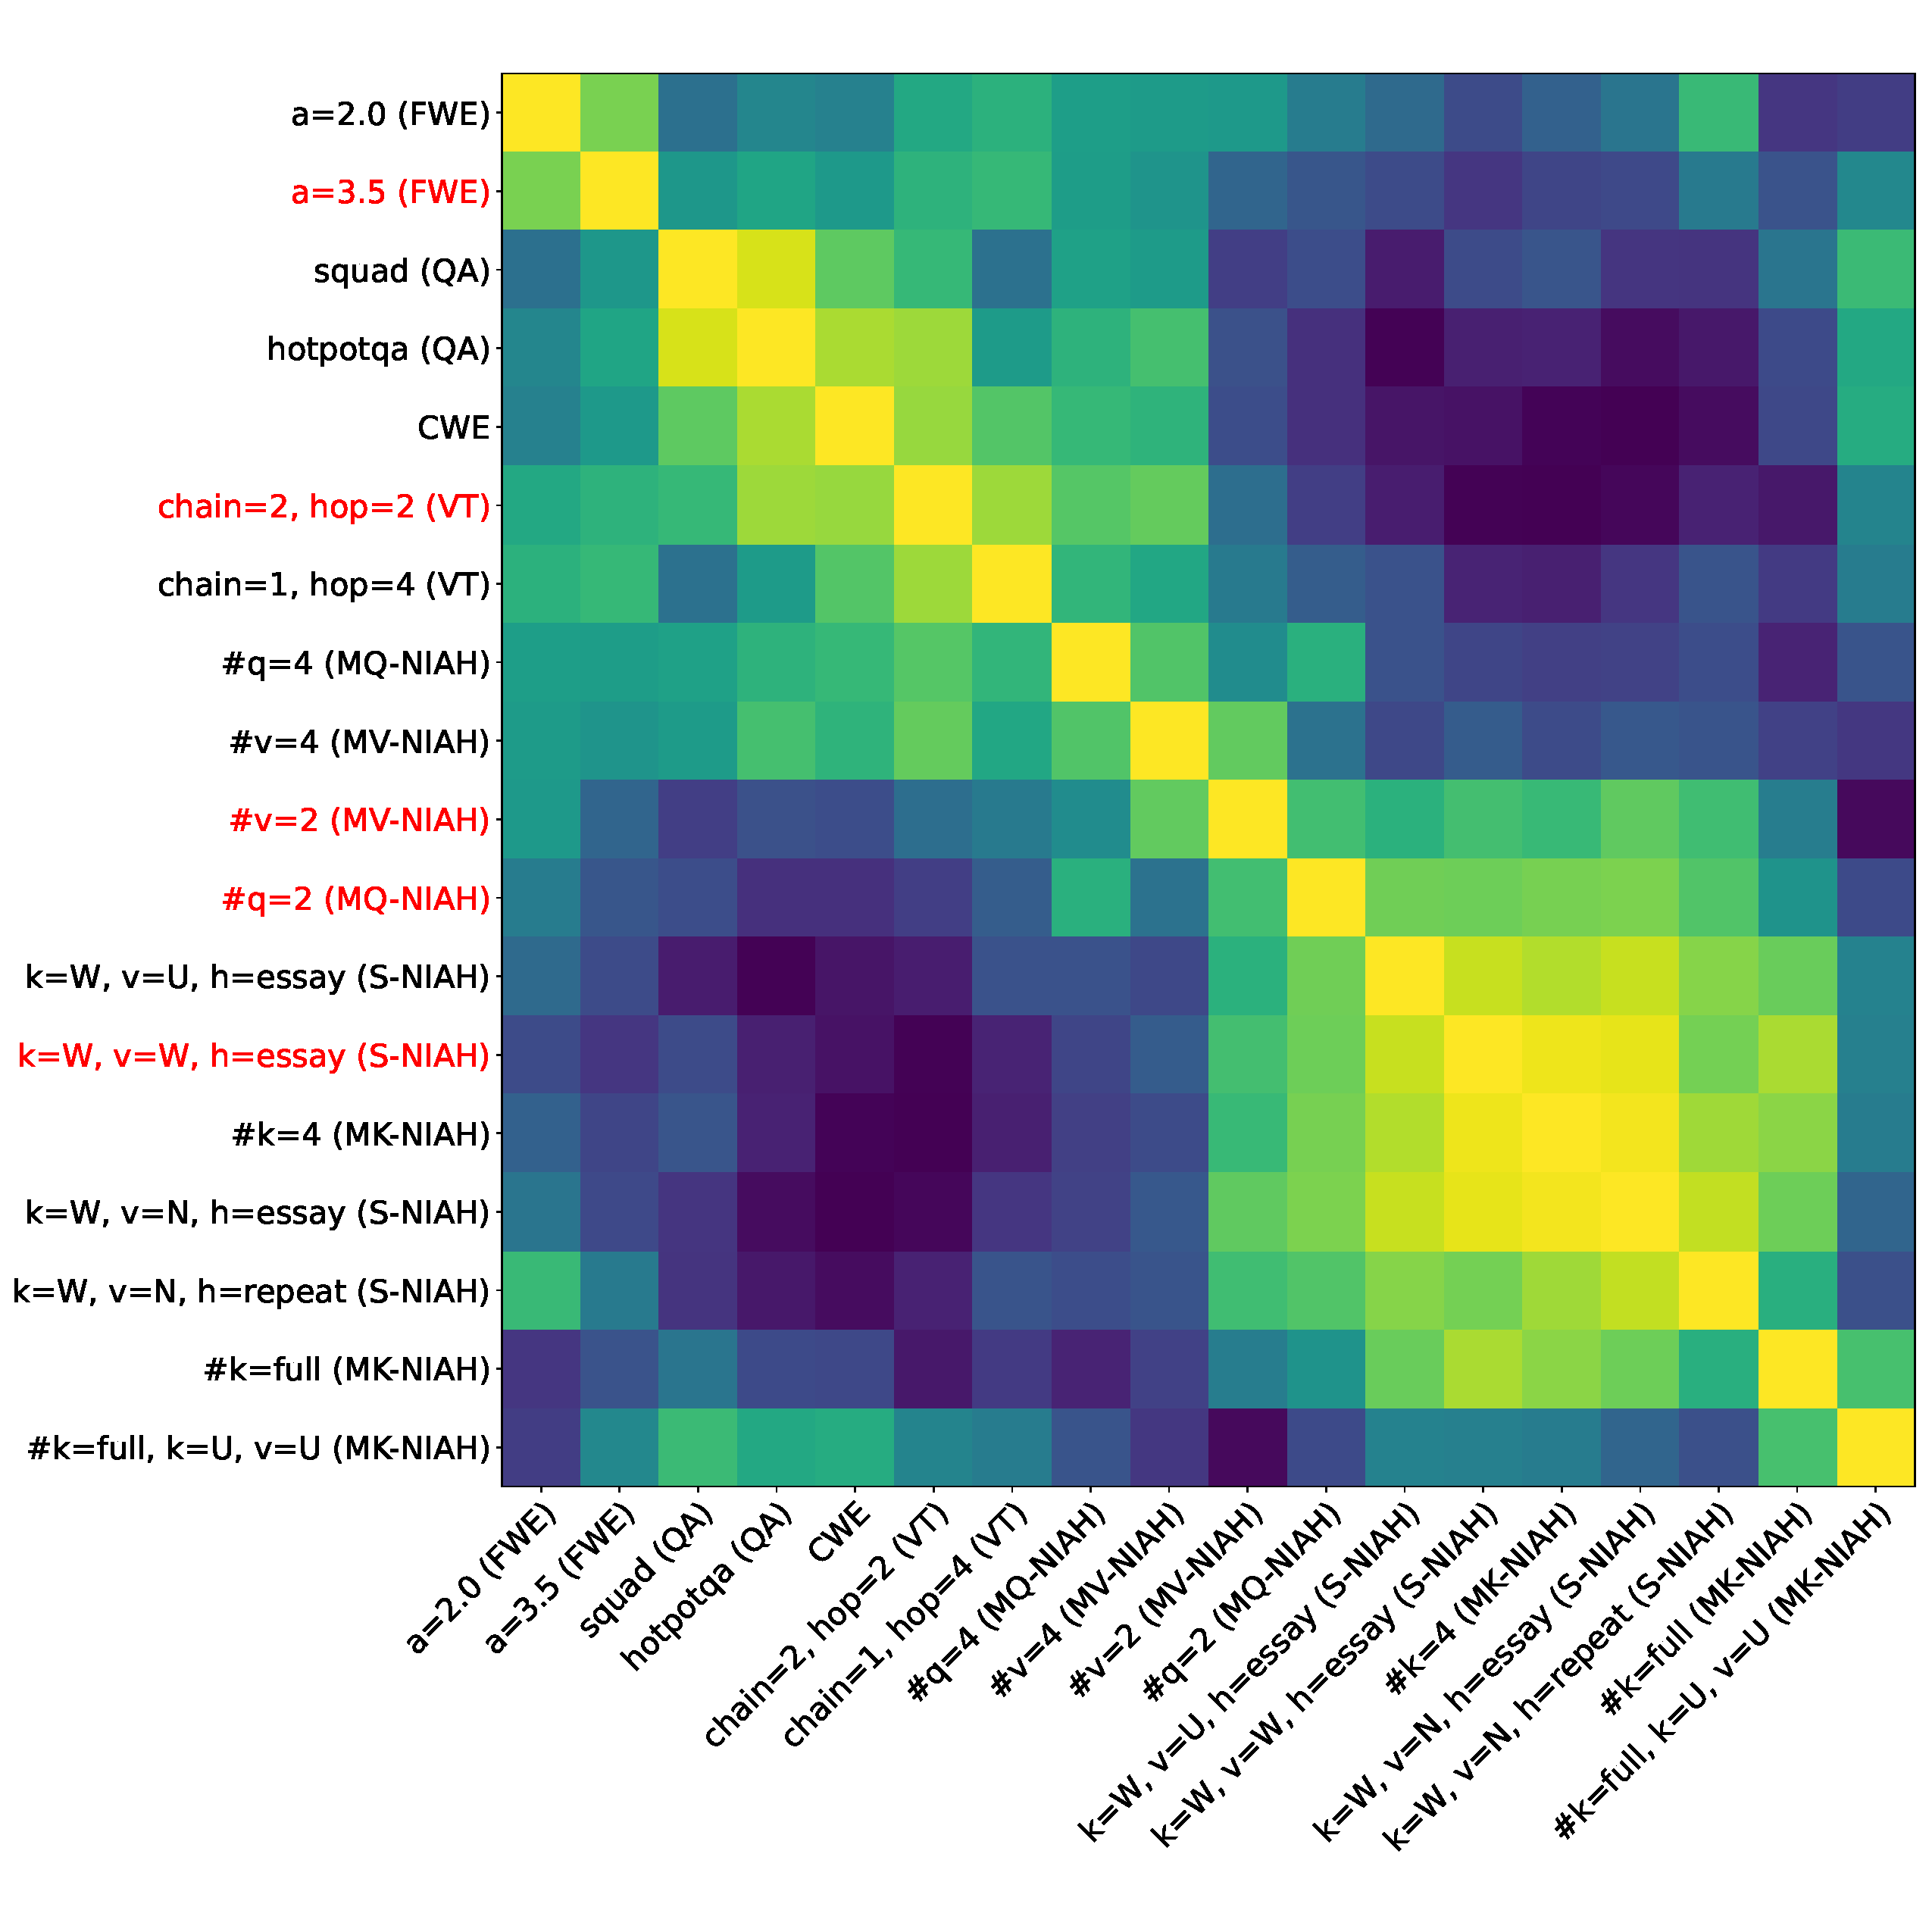
\includegraphics[width=\textwidth]{Image/pdf/corr_heatmap.pdf}
    \caption{Correlation heatmap among 18 tasks with diverse task configurations. We remove redundant tasks (in \textcolor{red}{red}) and only preserve 13 representative tasks in \ruler. (W: words; N: numbers; U: UUIDs; Full: entire haystack)}
    \label{fig:corr_heatmap}
\end{figure*}

\clearpage
\section{Prompt Templates}
\label{prompt_templates}
We decompose the input prompt template into the model template in Table~\ref{tab:model_template} and the task template in Table~\ref{tab:task_template1} \ref{tab:task_template2} \ref{tab:task_template3}. The model template is the model chat format while the task template combines instruction, context, and query. To prevent models from refusing to answer our questions, we append the input with an answer prefix to elicit model responses. For VT and CWE, we use one task sample as in-context demonstration.
\begin{table}[h]
    \centering
    \begin{tabular}{p{0.2\linewidth}p{0.7\linewidth}}
    \toprule
    \textbf{Model} & \textbf{Template} \\ 
    \midrule
    GPT-4 & \textcolor{violet}{\{task\_template\}} Do not provide any explanation. Please directly give me the answer. \textcolor{orange}{\{task\_answer\_prefix\}} \\
    \midrule
    Yi/Base & \textcolor{violet}{\{task\_template\}} \textcolor{orange}{\{task\_answer\_prefix\}} \\
    \midrule
    Command-R & 
    \begin{tabular}{@{}l@{}}
$\langle$BOS\_TOKEN$\rangle$\\$\langle|$START\_OF\_TURN\_TOKEN$|\rangle$\\$\langle|$USER\_TOKEN$|\rangle$\textcolor{violet}{\{task\_template\}}\\$\langle|$END\_OF\_TURN\_TOKEN$|\rangle$\\$\langle|$START\_OF\_TURN\_TOKEN$|\rangle$\\$\langle|$CHATBOT\_TOKEN$|\rangle$\textcolor{orange}{\{task\_answer\_prefix\}}
    \end{tabular}\\
    \midrule
    LWM/LongChat & \textcolor{red}{\{system\_prompt\}} USER: \textcolor{violet}{\{task\_template\}} ASSISTANT: \textcolor{orange}{\{task\_answer\_prefix\}} \\
    \midrule
    GLM & \begin{tabular}{@{}l@{}}[\,gMASK]\,sop$\langle|$user$|\rangle$\\ \textcolor{violet}{\{task\_template\}}$\langle|$assistant$|\rangle$\\ \textcolor{orange}{\{task\_answer\_prefix\}}\end{tabular}\\
    \midrule
    Phi3 & \begin{tabular}{@{}l@{}}$\langle|$user$|\rangle$\\\textcolor{violet}{\{task\_template\}}$\langle|$end$|\rangle$\\$\langle|$assistant$|\rangle$\\\textcolor{orange}{\{task\_answer\_prefix\}}\end{tabular}\\
    \midrule
    Qwen/DBRX & \begin{tabular}{@{}l@{}}$\langle|$im\_start$|\rangle$system\\\textcolor{red}{\{system\_prompt\}}$\langle|$im\_end$|\rangle$\\$\langle|$im\_start$|\rangle$user\\\textcolor{violet}{\{task\_template\}}$\langle|$im\_end$|\rangle$\\$\langle|$im\_start$|\rangle$assistant\\\textcolor{orange}{\{task\_answer\_prefix\}}\end{tabular}\\
    \midrule
    Llama3/Llama3.1 & \begin{tabular}{@{}l@{}}$\langle|$begin\_of\_text$|\rangle$$\langle|$start\_header\_id$|\rangle$user$\langle|$end\_header\_id$|\rangle$\\ \\ 
    \textcolor{violet}{\{task\_template\}}$\langle|$eot\_id$|\rangle$\\$\langle|$start\_header\_id$|\rangle$assistant$\langle|$end\_header\_id$|\rangle$\\ \\ \textcolor{orange}{\{task\_answer\_prefix\}}\end{tabular}\\
    \midrule
    Llama2/Others & [\,INST]\, \textcolor{violet}{\{task\_template\}} [\,/INST]\, \textcolor{orange}{\{task\_answer\_prefix\}} \\
    \bottomrule
    \end{tabular}
    \caption{Model chat templates. We append a task answer prefix in model response to prevent models from refusing to answer our questions. The addition of answer prefix does not break the models' chat template.}
    \label{tab:model_template}
\end{table}

\clearpage
\begin{table}[H]
    \small
    \centering
    \resizebox{\linewidth}{!}{
    \begin{tabular}{cp{0.9\linewidth}}
    \toprule
    
    \begin{tabular}{@{}c@{}}S-NIAH\\Subtask-1\end{tabular} & 
    \begin{tabular}{@{}p{\linewidth}@{}} 
    \textbf{Task Template:} \\
    Some special magic numbers are hidden within the following text. Make sure to memorize it. I will quiz you about the numbers afterwards.\\
    \textcolor{lightgray}{The grass is green. The sky is blue. The sun is yellow. Here we go. There and back again.} \\
    \textcolor{lightgray}{......} One of the special magic numbers for \textcolor{violet}{\{word\}} is: \textcolor{orange}{\{number\}}. \textcolor{lightgray}{......}\\
    What is the special magic number for \textcolor{violet}{\{word\}} mentioned in the provided text? \\ \\
    \textbf{Task Answer Prefix:} \\
    The special magic number for \textcolor{violet}{\{word\}} mentioned in the provided text is\end{tabular}\\

    \midrule

    \begin{tabular}{@{}c@{}}S-NIAH\\Subtask-2\end{tabular} & 
    \begin{tabular}{@{}p{\linewidth}@{}} 
    \textbf{Task Template:} \\
    Some special magic numbers are hidden within the following text. Make sure to memorize it. I will quiz you about the numbers afterwards.\\
    \textcolor{lightgray}{Paul Graham Essays.} \\
    \textcolor{lightgray}{......} One of the special magic numbers for \textcolor{violet}{\{word\}} is: \textcolor{orange}{\{number\}}. \textcolor{lightgray}{......}\\
    What is the special magic number for \textcolor{violet}{\{word\}} mentioned in the provided text? \\ \\
    \textbf{Task Answer Prefix:} \\
    The special magic number for \textcolor{violet}{\{word\}} mentioned in the provided text is\end{tabular}\\

    \midrule

    % \begin{tabular}{@{}c@{}}S-NIAH\\task3\end{tabular} & 
    % \begin{tabular}{@{}p{\linewidth}@{}} 
    % \textbf{Task Template:} \\
    % Some special magic uuids are hidden within the following text. Make sure to memorize it. I will quiz you about the uuids afterwards.\\
    % \textcolor{lightgray}{Paul Graham Essays.} \\
    % \textcolor{lightgray}{......} One of the special magic uuids for \textcolor{violet}{\{word\}} is: \textcolor{orange}{\{UUID\}}. \textcolor{lightgray}{......}\\
    % What is the special magic uuid for \textcolor{violet}{\{word\}} mentioned in the provided text? \\ \\
    % \textbf{Task Answer Prefix:} \\
    % The special magic uuid for \textcolor{violet}{\{word\}} mentioned in the provided text is\end{tabular}\\

    % \midrule

    \begin{tabular}{@{}c@{}}S-NIAH\\Subtask-3\end{tabular} & 
    \begin{tabular}{@{}p{\linewidth}@{}} 
    \textbf{Task Template:} \\
    Some special magic words are hidden within the following text. Make sure to memorize it. I will quiz you about the words afterwards.\\
    \textcolor{lightgray}{Paul Graham Essays.} \\
    \textcolor{lightgray}{......} One of the special magic words for \textcolor{violet}{\{word\}} is: \textcolor{orange}{\{word\}}. \textcolor{lightgray}{......}\\
    What is the special magic word for \textcolor{violet}{\{word\}} mentioned in the provided text? \\ \\
    \textbf{Task Answer Prefix:} \\
    The special magic word for \textcolor{violet}{\{word\}} mentioned in the provided text is\end{tabular}\\

    \midrule

    \begin{tabular}{@{}c@{}}MK-NIAH\\Subtask-1\end{tabular} & 
    \begin{tabular}{@{}p{\linewidth}@{}} 
    \textbf{Task Template:} \\
    Some special magic numbers are hidden within the following text. Make sure to memorize it. I will quiz you about the numbers afterwards.\\
    \textcolor{lightgray}{Paul Graham Essays.} \\
    \textcolor{lightgray}{......} \textcolor{lightgray}{One of the special magic numbers for \{word-1\} is: \{number-1\}.} \textcolor{lightgray}{......}\\
    \textcolor{lightgray}{......} \textcolor{lightgray}{One of the special magic numbers for \{word-2\} is: \{number-2\}.} \textcolor{lightgray}{......}\\
    \textcolor{lightgray}{......} \textcolor{lightgray}{One of the special magic numbers for \{word-3\} is: \{number-3\}.} \textcolor{lightgray}{......}\\
    \textcolor{lightgray}{......} One of the special magic numbers for \textcolor{violet}{\{word-4\}} is: \textcolor{orange}{\{number-4\}}. \textcolor{lightgray}{......}\\
    What is the special magic number for \textcolor{violet}{\{word-4\}} mentioned in the provided text? \\ \\
    \textbf{Task Answer Prefix:} \\
    The special magic number for \textcolor{violet}{\{word-4\}} mentioned in the provided text is\end{tabular}\\

    \midrule

    \begin{tabular}{@{}c@{}}MK-NIAH\\Subtask-2\end{tabular} & 
    \begin{tabular}{@{}p{\linewidth}@{}} 
    \textbf{Task Template:} \\
    Some special magic numbers are hidden within the following text. Make sure to memorize it. I will quiz you about the numbers afterwards.\\
    \textcolor{lightgray}{One of the special magic numbers for \{word-1\} is: \{number-1\}.} \\
    \textcolor{lightgray}{One of the special magic numbers for \{word-2\} is: \{number-2\}.} \\
    \textcolor{lightgray}{......} One of the special magic numbers for \textcolor{violet}{\{word-x\}} is: \textcolor{orange}{\{number-x\}}. \textcolor{lightgray}{......}\\
    \textcolor{lightgray}{One of the special magic numbers for \{word-n-1\} is: \{number-n-1\}.} \\
    \textcolor{lightgray}{One of the special magic numbers for \{word-n\} is: \{number-n\}.} \\
    What is the special magic number for \textcolor{violet}{\{word-x\}} mentioned in the provided text? \\ \\
    \textbf{Task Answer Prefix:} \\
    The special magic number for \textcolor{violet}{\{word-x\}} mentioned in the provided text is\end{tabular}\\

    \midrule

    \begin{tabular}{@{}c@{}}MK-NIAH\\Subtask-3\end{tabular} & 
    \begin{tabular}{@{}p{\linewidth}@{}} 
    \textbf{Task Template:} \\
    Some special magic uuids are hidden within the following text. Make sure to memorize it. I will quiz you about the uuids afterwards.\\
    \textcolor{lightgray}{One of the special magic uuids for \{uuid-1\} is: \{uuid-1\}.} \\
    \textcolor{lightgray}{One of the special magic uuids for \{uuid-2\} is: \{uuid-2\}.} \\
    \textcolor{lightgray}{......} One of the special magic uuids for \textcolor{violet}{\{uuid-x\}} is: \textcolor{orange}{\{uuid-x\}}. \textcolor{lightgray}{......}\\
    \textcolor{lightgray}{One of the special magic uuids for \{uuid-n-1\} is: \{uuid-n-1\}.} \\
    \textcolor{lightgray}{One of the special magic uuids for \{uuid-n\} is: \{uuid-n\}.} \\
    What is the special magic number for \textcolor{violet}{\{uuid-x\}} mentioned in the provided text? \\ \\
    \textbf{Task Answer Prefix:} \\
    The special magic number for \textcolor{violet}{\{uuid-x\}} mentioned in the provided text is\end{tabular}\\

    
    \bottomrule
    \end{tabular}}
    \caption{S-NIAH and MK-NIAH templates.}
    \label{tab:task_template1}
\end{table}




% \begin{table}[!h]
%     \small
%     \centering
%     \resizebox{\linewidth}{!}{
%     \begin{tabular}{cp{0.9\linewidth}}
%     \toprule
    
%     \begin{tabular}{@{}c@{}}MK-NIAH\\Subtask-1\end{tabular} & 
%     \begin{tabular}{@{}p{\linewidth}@{}} 
%     \textbf{Task Template:} \\
%     Some special magic numbers are hidden within the following text. Make sure to memorize it. I will quiz you about the numbers afterwards.\\
%     \textcolor{lightgray}{Paul Graham Essays.} \\
%     \textcolor{lightgray}{......} \textcolor{lightgray}{One of the special magic numbers for \{word-1\} is: \{number-1\}.} \textcolor{lightgray}{......}\\
%     \textcolor{lightgray}{......} \textcolor{lightgray}{One of the special magic numbers for \{word-2\} is: \{number-2\}.} \textcolor{lightgray}{......}\\
%     \textcolor{lightgray}{......} \textcolor{lightgray}{One of the special magic numbers for \{word-3\} is: \{number-3\}.} \textcolor{lightgray}{......}\\
%     \textcolor{lightgray}{......} One of the special magic numbers for \textcolor{violet}{\{word-4\}} is: \textcolor{orange}{\{number-4\}}. \textcolor{lightgray}{......}\\
%     What is the special magic number for \textcolor{violet}{\{word-4\}} mentioned in the provided text? \\ \\
%     \textbf{Task Answer Prefix:} \\
%     The special magic number for \textcolor{violet}{\{word-4\}} mentioned in the provided text is\end{tabular}\\

%     \midrule

%     \begin{tabular}{@{}c@{}}MK-NIAH\\Subtask-2\end{tabular} & 
%     \begin{tabular}{@{}p{\linewidth}@{}} 
%     \textbf{Task Template:} \\
%     Some special magic numbers are hidden within the following text. Make sure to memorize it. I will quiz you about the numbers afterwards.\\
%     \textcolor{lightgray}{One of the special magic numbers for \{word-1\} is: \{number-1\}.} \\
%     \textcolor{lightgray}{One of the special magic numbers for \{word-2\} is: \{number-2\}.} \\
%     \textcolor{lightgray}{......} One of the special magic numbers for \textcolor{violet}{\{word-x\}} is: \textcolor{orange}{\{number-x\}}. \textcolor{lightgray}{......}\\
%     \textcolor{lightgray}{One of the special magic numbers for \{word-n-1\} is: \{number-n-1\}.} \\
%     \textcolor{lightgray}{One of the special magic numbers for \{word-n\} is: \{number-n\}.} \\
%     What is the special magic number for \textcolor{violet}{\{word-x\}} mentioned in the provided text? \\ \\
%     \textbf{Task Answer Prefix:} \\
%     The special magic number for \textcolor{violet}{\{word-x\}} mentioned in the provided text is\end{tabular}\\

%     \midrule

%     \begin{tabular}{@{}c@{}}MK-NIAH\\Subtask-3\end{tabular} & 
%     \begin{tabular}{@{}p{\linewidth}@{}} 
%     \textbf{Task Template:} \\
%     Some special magic uuids are hidden within the following text. Make sure to memorize it. I will quiz you about the uuids afterwards.\\
%     \textcolor{lightgray}{One of the special magic uuids for \{uuid-1\} is: \{uuid-1\}.} \\
%     \textcolor{lightgray}{One of the special magic uuids for \{uuid-2\} is: \{uuid-2\}.} \\
%     \textcolor{lightgray}{......} One of the special magic uuids for \textcolor{violet}{\{uuid-x\}} is: \textcolor{orange}{\{uuid-x\}}. \textcolor{lightgray}{......}\\
%     \textcolor{lightgray}{One of the special magic uuids for \{uuid-n-1\} is: \{uuid-n-1\}.} \\
%     \textcolor{lightgray}{One of the special magic uuids for \{uuid-n\} is: \{uuid-n\}.} \\
%     What is the special magic number for \textcolor{violet}{\{uuid-x\}} mentioned in the provided text? \\ \\
%     \textbf{Task Answer Prefix:} \\
%     The special magic number for \textcolor{violet}{\{uuid-x\}} mentioned in the provided text is\end{tabular}\\
    
%     \bottomrule
%     \end{tabular}}
%     \caption{Multi-keys needle-in-a-haystack templates.}
%     \label{tab:task_template_mkniah}
% \end{table}




\begin{table}[H]
    \small
    \centering
    \resizebox{\linewidth}{!}{
    \begin{tabular}{cp{0.9\linewidth}}
    \toprule
    
    % \begin{tabular}{@{}c@{}}MV-NIAH\\Subtask-1\end{tabular} & 
    % \begin{tabular}{@{}p{\linewidth}@{}} 
    % \textbf{Task Template:} \\
    % Some special magic numbers are hidden within the following text. Make sure to memorize it. I will quiz you about the numbers afterwards.\\
    % \textcolor{lightgray}{Paul Graham Essays...} \\
    % \textcolor{lightgray}{......} One of the special magic numbers for \textcolor{violet}{\{word\}} is: \textcolor{orange}{\{number-1\}}. \textcolor{lightgray}{......}\\
    % \textcolor{lightgray}{......} One of the special magic numbers for \textcolor{violet}{\{word\}} is: \textcolor{orange}{\{number-2\}}. \textcolor{lightgray}{......}\\
    % What are all the special magic numbers for \textcolor{violet}{\{word\}} mentioned in the provided text? \\ \\
    % \textbf{Task Answer Prefix:} \\
    % The special magic numbers for \textcolor{violet}{\{word\}} mentioned in the provided text are\end{tabular}\\

    % \midrule

    \begin{tabular}{@{}c@{}}MV-NIAH\end{tabular} & 
    \begin{tabular}{@{}p{\linewidth}@{}} 
    \textbf{Task Template:} \\
    Some special magic numbers are hidden within the following text. Make sure to memorize it. I will quiz you about the numbers afterwards.\\
    \textcolor{lightgray}{Paul Graham Essays.} \\
    \textcolor{lightgray}{......} One of the special magic numbers for \textcolor{violet}{\{word\}} is: \textcolor{orange}{\{number-1\}}. \textcolor{lightgray}{......}\\
    \textcolor{lightgray}{......} One of the special magic numbers for \textcolor{violet}{\{word\}} is: \textcolor{orange}{\{number-2\}}. \textcolor{lightgray}{......}\\
    \textcolor{lightgray}{......} One of the special magic numbers for \textcolor{violet}{\{word\}} is: \textcolor{orange}{\{number-3\}}. \textcolor{lightgray}{......}\\
    \textcolor{lightgray}{......} One of the special magic numbers for \textcolor{violet}{\{word\}} is: \textcolor{orange}{\{number-4\}}. \textcolor{lightgray}{......}\\
    What are all the special magic numbers for \textcolor{violet}{\{word\}} mentioned in the provided text? \\ \\
    \textbf{Task Answer Prefix:} \\
    The special magic numbers for \textcolor{violet}{\{word\}} mentioned in the provided text are\end{tabular}\\

    \midrule

    % \begin{tabular}{@{}c@{}}MQ-NIAH\\Subtask-1\end{tabular} & 
    % \begin{tabular}{@{}p{\linewidth}@{}} 
    % \textbf{Task Template:} \\
    % Some special magic numbers are hidden within the following text. Make sure to memorize it. I will quiz you about the numbers afterwards.\\
    % \textcolor{lightgray}{Paul Graham Essays.} \\
    % \textcolor{lightgray}{......} One of the special magic numbers for \textcolor{violet}{\{word-1\}} is: \textcolor{orange}{\{number-1\}}. \textcolor{lightgray}{......} \\
    % \textcolor{lightgray}{......} One of the special magic numbers for \textcolor{violet}{\{word-2\}} is: \textcolor{orange}{\{number-2\}}. \textcolor{lightgray}{......}\\
    % What are all the special magic numbers for \textcolor{violet}{\{word-1\}} and \textcolor{violet}{\{word-2\}} mentioned in the provided text? \\ \\
    % \textbf{Task Answer Prefix:} \\
    % The special magic numbers for \textcolor{violet}{\{word-1\}} and \textcolor{violet}{\{word-2\}} mentioned in the provided text are\end{tabular}\\
    
    % \midrule
    
    \begin{tabular}{@{}c@{}}MQ-NIAH\end{tabular} & 
    \begin{tabular}{@{}p{\linewidth}@{}} 
    \textbf{Task Template:} \\
    Some special magic numbers are hidden within the following text. Make sure to memorize it. I will quiz you about the numbers afterwards.\\
    \textcolor{lightgray}{Paul Graham Essays.} \\
    \textcolor{lightgray}{......} One of the special magic numbers for \textcolor{violet}{\{word-1\}} is: \textcolor{orange}{\{number-1\}}. \textcolor{lightgray}{......} \\    
    \textcolor{lightgray}{......} One of the special magic numbers for \textcolor{violet}{\{word-2\}} is: \textcolor{orange}{\{number-2\}}. \textcolor{lightgray}{......} \\
    \textcolor{lightgray}{......} One of the special magic numbers for \textcolor{violet}{\{word-3\}} is: \textcolor{orange}{\{number-3\}}. \textcolor{lightgray}{......} \\
    \textcolor{lightgray}{......} One of the special magic numbers for \textcolor{violet}{\{word-4\}} is: \textcolor{orange}{\{number-4\}}. \textcolor{lightgray}{......}\\
    What are all the special magic numbers for \textcolor{violet}{\{word-1\}}, \textcolor{violet}{\{word-2\}}, \textcolor{violet}{\{word-3\}}, and \textcolor{violet}{\{word-4\}} mentioned in the provided text? \\ \\
    \textbf{Task Answer Prefix:} \\
    The special magic numbers for \textcolor{violet}{\{word-1\}}, \textcolor{violet}{\{word-2\}}, \textcolor{violet}{\{word-3\}}, and \textcolor{violet}{\{word-4\}} mentioned in the provided text are\end{tabular}\\

    \midrule

    \begin{tabular}{@{}c@{}}VT\end{tabular} & 
    \begin{tabular}{@{}p{\linewidth}@{}} 
    \textbf{Task Template:} \\
    \textcolor{blue}{\{one task example\}} \\
    Memorize and track the chain(s) of variable assignment hidden in the following text.\\\\
    \textcolor{lightgray}{The grass is green. The sky is blue. The sun is yellow. Here we go. There and back again.}
    \textcolor{lightgray}{......} VAR \textcolor{orange}{\{X1\}} = \textcolor{violet}{\{number\}} \textcolor{lightgray}{......}\\
    \textcolor{lightgray}{......} VAR \textcolor{orange}{\{X2\}} = \textcolor{orange}{\{X1\}} \textcolor{lightgray}{......}\\
    \textcolor{lightgray}{......} VAR \textcolor{orange}{\{X3\}} = \textcolor{orange}{\{X2\}} \textcolor{lightgray}{......}\\
    \textcolor{lightgray}{......} VAR \textcolor{orange}{\{X4\}} = \textcolor{orange}{\{X3\}} \textcolor{lightgray}{......}\\
    \textcolor{lightgray}{......} VAR \textcolor{orange}{\{X5\}} = \textcolor{orange}{\{X4\}} \textcolor{lightgray}{......}\\
   Question: Find all variables that are assigned the value \textcolor{violet}{\{number\}} in the text above. \\\\
    \textbf{Task Answer Prefix:} \\
    Answer: According to the chain(s) of variable assignment in the text above, 5 variables are assigned the value \textcolor{violet}{\{number\}}, they are: 
    \end{tabular}\\

    \midrule

    \begin{tabular}{@{}c@{}}CWE\end{tabular} & 
    \begin{tabular}{@{}p{\linewidth}@{}} 
    \textbf{Task Template:} \\
    \textcolor{blue}{\{one task example\}} \\
   Below is a numbered list of words. In these words, some appear more often than others. Memorize the ones that appear most often.\\
   1. \textcolor{orange}{word-a} 2. \textcolor{lightgray}{word-b} 3. \textcolor{lightgray}{word-c} 4. \textcolor{orange}{word-a} 5. \textcolor{lightgray}{word-d} 6. \textcolor{orange}{word-a} 7. \textcolor{lightgray}{word-e} 8. \textcolor{lightgray}{word-f} \textcolor{lightgray}{......}\\
   Question: What are the 10 most common words in the above list? \\\\
    \textbf{Task Answer Prefix:} \\
    Answer: The top 10 words that appear most often in the list are: 
    \end{tabular}\\

    \midrule

    \begin{tabular}{@{}c@{}}FWE\end{tabular} & 
    \begin{tabular}{@{}p{\linewidth}@{}} 
    \textbf{Task Template:} \\
    Read the following coded text and track the frequency of each coded word. Find the three most frequently appeared coded words. \textcolor{lightgray}{... ...} \textcolor{orange}{word-a} \textcolor{lightgray}{... word-b ... ... ... word-c ...} \textcolor{orange}{word-a} \textcolor{lightgray}{... word-d word-e ...} \textcolor{orange}{word-a} \textcolor{lightgray}{... ... word-f ... ... ... ... word-g ... word-h ...} \textcolor{orange}{word-a} \textcolor{lightgray}{... word-i ......} \\
    Question: Do not provide any explanation. Please ignore the dots '....'. What are the three most frequently appeared words in the above coded text? \\\\
    \textbf{Task Answer Prefix:} \\
    Answer: According to the coded text above, the three most frequently appeared words are:
    \end{tabular}\\
    
    \bottomrule
    \end{tabular}}
    \caption{MV-NIAH, MQ-NIAH, VT, CWE, and FWE templates.}
    \label{tab:task_template2}
\end{table}




% \begin{table}[!h]
%     \small
%     \centering
%     \resizebox{\linewidth}{!}{
%     \begin{tabular}{cp{0.9\linewidth}}
%     \toprule
    
%     \begin{tabular}{@{}c@{}}VT\end{tabular} & 
%     \begin{tabular}{@{}p{\linewidth}@{}} 
%     \textbf{Task Template:} \\
%     \textcolor{blue}{\{one task example\}} \\
%     Memorize and track the chain(s) of variable assignment hidden in the following text.\\\\
%     \textcolor{lightgray}{The grass is green. The sky is blue. The sun is yellow. Here we go. There and back again.}
%     \textcolor{lightgray}{......} VAR \textcolor{orange}{\{X1\}} = \textcolor{violet}{\{number\}} \textcolor{lightgray}{......}\\
%     \textcolor{lightgray}{......} VAR \textcolor{orange}{\{X2\}} = \textcolor{orange}{\{X1\}} \textcolor{lightgray}{......}\\
%     \textcolor{lightgray}{......} VAR \textcolor{orange}{\{X3\}} = \textcolor{orange}{\{X2\}} \textcolor{lightgray}{......}\\
%     \textcolor{lightgray}{......} VAR \textcolor{orange}{\{X4\}} = \textcolor{orange}{\{X3\}} \textcolor{lightgray}{......}\\
%     \textcolor{lightgray}{......} VAR \textcolor{orange}{\{X5\}} = \textcolor{orange}{\{X4\}} \textcolor{lightgray}{......}\\
%    Question: Find all variables that are assigned the value \textcolor{violet}{\{number\}} in the text above. \\\\
%     \textbf{Task Answer Prefix:} \\
%     Answer: According to the chain(s) of variable assignment in the text above, 5 variables are assigned the value \textcolor{violet}{\{number\}}, they are: 
%     \end{tabular}\\

   %  \midrule

   %  \begin{tabular}{@{}c@{}}VT\\task2\end{tabular} & 
   %  \begin{tabular}{@{}p{\linewidth}@{}} 
   %  \textbf{Task Template:} \\
   %  \textcolor{blue}{\{one task example\}} \\
   %  Memorize and track the chain(s) of variable assignment hidden in the following text.\\\\
   %  \textcolor{lightgray}{The grass is green. The sky is blue. The sun is yellow. Here we go. There and back again.}
   %  \textcolor{lightgray}{......} VAR \textcolor{orange}{\{X1\}} = \textcolor{violet}{\{numberX\}} \textcolor{lightgray}{......}\\
   %  \textcolor{lightgray}{...... VAR Y1 = numberY ......}\\
   %  \textcolor{lightgray}{......} VAR \textcolor{orange}{\{X2\}} = \textcolor{orange}{\{X1\}} \textcolor{lightgray}{......}\\
   %  \textcolor{lightgray}{...... VAR Y2 = Y1 ......}\\
   %  \textcolor{lightgray}{......} VAR \textcolor{orange}{\{X3\}} = \textcolor{orange}{\{X2\}} \textcolor{lightgray}{......}\\
   %  \textcolor{lightgray}{...... VAR Y3 = Y2 ......}\\
   % Question: Find all variables that are assigned the value \textcolor{violet}{\{numberX\}} in the text above. \\\\
   %  \textbf{Task Answer Prefix:} \\
   %  Answer: According to the chain(s) of variable assignment in the text above, 3 variables are assigned the value \textcolor{violet}{\{numberX\}}, they are: 
   %  \end{tabular}\\

%     \bottomrule
%     \end{tabular}}
%     \caption{Variable tracking templates.}
%     \label{tab:task_template_vt}
% \end{table}




% \begin{table}[!h]
%     \small
%     \centering
%     \resizebox{\linewidth}{!}{
%     \begin{tabular}{cp{0.9\linewidth}}
%     \toprule
    
%     \begin{tabular}{@{}c@{}}CWE\end{tabular} & 
%     \begin{tabular}{@{}p{\linewidth}@{}} 
%     \textbf{Task Template:} \\
%     \textcolor{blue}{\{one task example\}} \\
%    Below is a numbered list of words. In these words, some appear more often than others. Memorize the ones that appear most often.\\
%    1. \textcolor{orange}{word-a} 2. \textcolor{lightgray}{word-b} 3. \textcolor{lightgray}{word-c} 4. \textcolor{orange}{word-a} 5. \textcolor{lightgray}{word-d} 6. \textcolor{orange}{word-a} 7. \textcolor{lightgray}{word-e} 8. \textcolor{lightgray}{word-f} \textcolor{lightgray}{......}\\
%    Question: What are the 10 most common words in the above list? \\\\
%     \textbf{Task Answer Prefix:} \\
%     Answer: The top 10 words that appear most often in the list are: 
%     \end{tabular}\\

%     \midrule

%     \begin{tabular}{@{}c@{}}FWE\end{tabular} & 
%     \begin{tabular}{@{}p{\linewidth}@{}} 
%     \textbf{Task Template:} \\
%     Read the following coded text and track the frequency of each coded word. Find the three most frequently appeared coded words. \textcolor{lightgray}{... ...} \textcolor{orange}{word-a} \textcolor{lightgray}{... word-b ... ... ... word-c ...} \textcolor{orange}{word-a} \textcolor{lightgray}{... word-d word-e ...} \textcolor{orange}{word-a} \textcolor{lightgray}{... ... word-f ... ... ... ... word-g ... word-h ...} \textcolor{orange}{word-a} \textcolor{lightgray}{... word-i ......} \\
%     Question: Do not provide any explanation. Please ignore the dots '....'. What are the three most frequently appeared words in the above coded text? \\\\
%     \textbf{Task Answer Prefix:} \\
%     Answer: According to the coded text above, the three most frequently appeared words are:
%     \end{tabular}\\


%     \bottomrule
%     \end{tabular}}
%     \caption{Common and frequent word extraction templates.}
%     \label{tab:task_template_ag}
% \end{table}




\begin{table}[H]
    \small
    \centering
    \resizebox{\linewidth}{!}{
    \begin{tabular}{cp{0.9\linewidth}}
    \toprule
    
    \begin{tabular}{@{}c@{}}Single\\Hop\\QA\end{tabular} & 
    \begin{tabular}{@{}p{\linewidth}@{}} 
    \textbf{Task Template:} \\
    Answer the question based on the given documents. Only give me the answer and do not output any other words.\\\\
    The following are given documents.\\\\
    \textcolor{lightgray}{Document 1:} \\ \textcolor{lightgray}{\{document-1\}} \\
    \textcolor{lightgray}{......} \\
    \textcolor{violet}{Document x:} \\ \textcolor{orange}{\{document-x\}} \\
    \textcolor{lightgray}{......} \\
    \textcolor{lightgray}{Document n:} \\ \textcolor{lightgray}{\{document-n\}} \\\\
    
    Answer the question based on the given documents. Only give me the answer and do not output any other words.\\\\
    Question: \textcolor{violet}{question}\\\\
    \textbf{Task Answer Prefix:} \\
    Answer: 
    \end{tabular}\\

    \midrule

    \begin{tabular}{@{}c@{}}Multi\\Hop\\QA\end{tabular} & 
    \begin{tabular}{@{}p{\linewidth}@{}} 
    \textbf{Task Template:} \\
    Answer the question based on the given documents. Only give me the answer and do not output any other words.\\\\
    The following are given documents.\\\\
    \textcolor{lightgray}{Document 1:} \\ \textcolor{lightgray}{\{document-1\}} \\
    \textcolor{lightgray}{......} \\
    \textcolor{violet}{Document x:} \\ \textcolor{orange}{\{document-x\}} \\
    \textcolor{lightgray}{......} \\
    \textcolor{violet}{Document y:} \\ \textcolor{orange}{\{document-y\}} \\
    \textcolor{lightgray}{......} \\
    \textcolor{lightgray}{Document n:} \\ \textcolor{lightgray}{\{document-n\}} \\\\
    
    Answer the question based on the given documents. Only give me the answer and do not output any other words.\\\\
    Question: \textcolor{violet}{question}\\\\
    \textbf{Task Answer Prefix:} \\
    Answer: 
    \end{tabular}\\
    
    \bottomrule
    \end{tabular}}
    \caption{QA templates.}
    \label{tab:task_template3}
\end{table}

\clearpage
\section{Passkey Retrieval and Vanilla NIAH Results}
\label{perfect_results}
% \begin{table}[H]
\resizebox{\linewidth}{!}{
\begin{tabular}{@{}l|c|cccccc|c@{}}
\toprule

\bf Models & \begin{tabular}{@{}c@{}}\bf \small Claimed\\\bf \small Length\end{tabular} & \bf4k & \bf8k & \bf16k & \bf32k & \bf64k & \bf128k & \begin{tabular}{@{}c@{}}\bf Avg.\end{tabular} \\

\midrule

GPT-4 & 128k & 100.0 & 100.0 & 100.0 & 100.0 & 100.0 & 100.0 & 100.0 \\
Command-R (35B) & 128k & 100.0 & 100.0 & 100.0 & 100.0 & 100.0 & 100.0 & 100.0 \\
Yi (34B) & 200k & 100.0 & 100.0 & 100.0 & 100.0 & 100.0 & 100.0 & 100.0 \\
Mixtral (8x7B) & 32k & 100.0 & 100.0 & 100.0 & 100.0 & 100.0 & 97.0 & 99.5 \\
Mistral (7B) & 32k & 100.0 & 100.0 & 100.0 & 100.0 & 99.6 & 69.6 & 94.9 \\
ChatGLM (6B) & 128k & 100.0 & 100.0 & 100.0 & 100.0 & 100.0 & 100.0 & 100.0 \\
LWM (7B) & 1M & 100.0 & 100.0 & 100.0 & 100.0 & 100.0 & 100.0 & 100.0 \\
Together (7B) & 32k & 100.0 & 100.0 & 100.0 & 100.0 & 0.0 & 0.0 & 66.7 \\
LongChat (7B) & 32k & 100.0 & 100.0 & 100.0 & 99.4 & 0.0 & 0.0 & 66.6 \\
LongAlpaca (13B)& 32k & 88.2 & 88.6 & 86.4 & 82.4 & 0.0 & 0.0 & 57.6 \\


\midrule
\midrule

Mixtral-base (8x7B) & 32k & 100.0 & 100.0 & 100.0 & 100.0 & 100.0 & 46.8 & 91.1 \\
Mistral-base (7B) & 32k & 100.0 & 100.0 & 100.0 & 100.0 & 99.6 & 70.8 & 95.1 \\
Jamba-base (52B) & 256k & 100.0 & 100.0 & 100.0 & 100.0 & 100.0 & 100.0 & 100.0 \\
LWM-base (7B) & 1M & 99.8 & 100.0 & 99.6 & 99.6 & 98.2 & 96.0 & 98.9 \\
LongLoRA-base (7B) & 100k & 99.6 & 99.4 & 99.0 & 99.4 & 99.4 & 0.0 & 82.8 \\
Yarn-base (7B) & 128k & 100.0 & 100.0 & 99.0 & 100.0 & 99.2 & 39.6 & 89.6 \\
Together-base (7B) & 32k & 100.0 & 100.0 & 99.8 & 100.0 & 0.0 & 0.0 & 66.6 \\

\bottomrule
\end{tabular}}
\caption{Performance of selected aligned and base models across length 4k to 128k in passkey retrieval of \ruler. Almost all models have perfect score at their claimed length.}
\label{tab:main_result_passkey}
\end{table}










\begin{table}[h]
\resizebox{\linewidth}{!}{
\begin{tabular}{@{}l|c|cccccc|c@{}}
\toprule

\bf Models & \begin{tabular}{@{}c@{}}\bf \small Claimed\\\bf \small Length\end{tabular} & \bf4k & \bf8k & \bf16k & \bf32k & \bf64k & \bf128k & \begin{tabular}{@{}c@{}}\bf Avg.\end{tabular} \\

\midrule

GPT-4 & 128k & 100.0 & 100.0 & 100.0 & 100.0 & 100.0 & 100.0 & 100.0 \\
Command-R (35B) & 128k & 100.0 & 100.0 & 100.0 & 100.0 & 100.0 & 98.0 & 99.7 \\
Yi (34B) & 200k & 100.0 & 100.0 & 100.0 & 100.0 & 100.0 & 100.0 & 100.0 \\
Mixtral (8x7B) & 32k & 100.0 & 100.0 & 100.0 & 100.0 & 93.2 & 43.8 & 89.5 \\
Mistral (7B) & 32k & 100.0 & 100.0 & 100.0 & 97.0 & 70.0 & 7.4 & 79.1 \\
ChatGLM (6B) & 128k & 100.0 & 100.0 & 99.0 & 99.6 & 90.8 & 87.0 & 96.1 \\
LWM (7B) & 1M & 100.0 & 100.0 & 100.0 & 100.0 & 100.0 & 100.0 & 100.0 \\
Together (7B) & 32k & 100.0 & 100.0 & 100.0 & 99.8 & 0.0 & 0.0 & 66.7 \\
LongChat (7B) & 32k & 100.0 & 100.0 & 97.6 & 98.4 & 0.0 & 0.0 & 66.0 \\
LongAlpaca (13B) & 32k & 90.2 & 90.2 & 88.4 & 83.4 & 0.0 & 0.0 & 58.7 \\

\midrule
\midrule

Mixtral-base (8x7B) & 32k & 100.0 & 100.0 & 100.0 & 100.0 & 85.2 & 34.8 & 86.7 \\
Mistral-base (7B) & 32k & 100.0 & 100.0 & 100.0 & 100.0 & 94.8 & 0.4 & 82.5 \\
Jamba-base (52B) & 256k & 100.0 & 100.0 & 98.8 & 99.8 & 99.8 & 86.4 & 97.5 \\
LWM-base (7B) & 1M & 100.0 & 99.4 & 97.8 & 98.6 & 98.2 & 98.6 & 98.8 \\
LongLoRA-base (7B) & 100k & 99.8 & 100.0 & 100.0 & 99.8 & 100.0 & 0.0 & 83.3 \\
Yarn-base (7B) & 128k & 97.4 & 97.8 & 91.4 & 85.4 & 86.6 & 20.0 & 79.8 \\
Together-base (7B) & 32k & 100.0 & 100.0 & 100.0 & 99.8 & 0.0 & 0.0 & 66.6 \\

\bottomrule
\end{tabular}}
\caption{Performance of selected aligned and base models across length 4k to 128k in vanilla NIAH of \ruler. Almost all models have perfect score at their claimed length.}
\label{tab:main_result_passkey_2}
\end{table}
\begin{table}[H]
\centering
\resizebox{0.85\linewidth}{!}{
\begin{tabular}{@{}l|c|cccccc|c@{}}
\toprule

\bf Models & \begin{tabular}{@{}c@{}}\bf \small Claimed\\\bf \small Length\end{tabular} & \bf4K & \bf8K & \bf16K & \bf32K & \bf64K & \bf128K & \begin{tabular}{@{}c@{}}\bf Avg.\end{tabular} \\

\midrule
Gemini-1.5 & 1M & 100.0 & 100.0 & 100.0 & 100.0 & 100.0 & 100.0 & 100.0 \\
GPT-4 & 128K & 100.0 & 100.0 & 100.0 & 100.0 & 100.0 & 100.0 & 100.0 \\
Llama3.1 (70B) & 128K & 100.0 & 100.0 & 100.0 & 100.0 & 100.0 & 97.8 & 99.6 \\
Llama3.1 (8B) & 128K & 100.0 & 100.0 & 100.0 & 100.0 & 100.0 & 100.0 & 100.0 \\
Qwen2 (72B) & 128K & 100.0 & 100.0 & 100.0 & 100.0 & 100.0 & 96.6 & 99.4 \\
Command-R-plus (104B) & 128K & 100.0 & 100.0 & 99.8 & 99.8 & 100.0 & 97.2 & 99.5 \\
GLM4 (9B) & 1M & 100.0 & 100.0 & 100.0 & 100.0 & 100.0 & 100.0 & 100.0 \\
GradientAI/Llama3 (70B) & 1M & 100.0 & 100.0 & 100.0 & 100.0 & 100.0 & 93.6 & 98.9 \\
Mixtral-8x22B (39B/141B) & 64K & 100.0 & 100.0 & 100.0 & 100.0 & 99.6 & 0.0 & 83.3 \\
Yi (34B) & 200K & 100.0 & 100.0 & 100.0 & 100.0 & 100.0 & 100.0 & 100.0 \\
Phi3-medium (14B) & 128K & 100.0 & 100.0 & 100.0 & 100.0 & 100.0 & 88.0 & 98.0 \\
Mistral-v0.2 (7B) & 32K & 100.0 & 100.0 & 100.0 & 100.0 & 99.6 & 69.6 & 94.9 \\
LWM (7B) & 1M & 100.0 & 100.0 & 100.0 & 100.0 & 100.0 & 100.0 & 100.0 \\
DBRX (36B/132B) & 32K & 100.0 & 100.0 & 100.0 & 100.0 & 0.0 & 0.0 & 66.7 \\
Together (7B) & 32K & 100.0 & 100.0 & 100.0 & 100.0 & 0.0 & 0.0 & 66.7 \\
LongChat (7B) & 32K & 100.0 & 100.0 & 100.0 & 99.4 & 0.0 & 0.0 & 66.6 \\
LongAlpaca (13B)& 32K & 88.2 & 88.6 & 86.4 & 82.4 & 0.0 & 0.0 & 57.6 \\


\midrule
\midrule

Mixtral-base (8x7B) & 32K & 100.0 & 100.0 & 100.0 & 100.0 & 100.0 & 46.8 & 91.1 \\
Mistral-base (7B) & 32K & 100.0 & 100.0 & 100.0 & 100.0 & 99.6 & 70.8 & 95.1 \\
Jamba-base (52B) & 256K & 100.0 & 100.0 & 100.0 & 100.0 & 100.0 & 100.0 & 100.0 \\
LWM-base (7B) & 1M & 99.8 & 100.0 & 99.6 & 99.6 & 98.2 & 96.0 & 98.9 \\
LongLoRA-base (7B) & 100K & 99.6 & 99.4 & 99.0 & 99.4 & 99.4 & 0.0 & 82.8 \\
Yarn-base (7B) & 128K & 100.0 & 100.0 & 99.0 & 100.0 & 99.2 & 39.6 & 89.6 \\
Together-base (7B) & 32K & 100.0 & 100.0 & 99.8 & 100.0 & 0.0 & 0.0 & 66.6 \\

\bottomrule
\end{tabular}}
\caption{Performance of selected aligned and base models across length 4K to 128K in passkey retrieval of \ruler. Almost all models have perfect score at their claimed length.}
\label{tab:main_result_passkey}
\end{table}










\begin{table}[h]
\centering
\resizebox{0.85\linewidth}{!}{
\begin{tabular}{@{}l|c|cccccc|c@{}}
\toprule

\bf Models & \begin{tabular}{@{}c@{}}\bf \small Claimed\\\bf \small Length\end{tabular} & \bf4K & \bf8K & \bf16K & \bf32K & \bf64K & \bf128K & \begin{tabular}{@{}c@{}}\bf Avg.\end{tabular} \\

\midrule
Gemini-1.5 & 1M & 100.0 & 100.0 & 100.0 & 98.0 & 100.0 & 100.0 & 99.7 \\
GPT-4 & 128K & 100.0 & 100.0 & 100.0 & 100.0 & 100.0 & 100.0 & 100.0 \\
Llama3.1 (70B) & 128K & 100.0 & 100.0 & 100.0 & 100.0 & 100.0 & 99.6 & 99.9 \\
Llama3.1 (8B) & 128K & 100.0 & 100.0 & 100.0 & 100.0 & 100.0 & 99.6 & 99.9 \\
Qwen2 (72B) & 128K & 100.0 & 100.0 & 100.0 & 100.0 & 99.8 & 56.4 & 92.7 \\
Command-R-plus (35B) & 128K & 100.0 & 100.0 & 100.0 & 100.0 & 99.8 & 86.0 & 97.6 \\
GLM4 (9B) & 128K & 100.0 & 100.0 & 100.0 & 100.0 & 100.0 & 100.0 & 100.0 \\
GradientAI/Llama3 (70B) & 1M & 100.0 & 100.0 & 100.0 & 99.6 & 99.2 & 97.8 & 99.4 \\
Mixtral-8x22B (39B/141B) & 64K & 100.0 & 100.0 & 100.0 & 100.0 & 99.6 & 24.2 & 87.3 \\
Yi (34B) & 200K & 100.0 & 100.0 & 100.0 & 100.0 & 100.0 & 100.0 & 100.0 \\
Phi3-medium (14B) & 128K & 100.0 & 99.8 & 100.0 & 99.8 & 99.8 & 73.8 & 95.5 \\
Mistral-v0.2 (7B) & 32K & 100.0 & 100.0 & 100.0 & 97.0 & 70.0 & 7.4 & 79.1 \\
LWM (7B) & 1M & 100.0 & 100.0 & 100.0 & 100.0 & 100.0 & 100.0 & 100.0 \\
DBRX (36B/132B) & 32K & 100.0 & 100.0 & 90.0 & 93.2 & 0.8 & 0.0 & 64.0 \\
Together (7B) & 32K & 100.0 & 100.0 & 100.0 & 99.8 & 0.0 & 0.0 & 66.6 \\
LongChat (7B) & 32K & 100.0 & 100.0 & 97.6 & 98.4 & 0.0 & 0.0 & 66.0 \\
LongAlpaca (13B) & 32K & 90.2 & 90.2 & 88.4 & 83.4 & 0.0 & 0.0 & 58.7 \\

\midrule
\midrule

Mixtral-base (8x7B) & 32K & 100.0 & 100.0 & 100.0 & 100.0 & 85.2 & 34.8 & 86.7 \\
Mistral-base (7B) & 32K & 100.0 & 100.0 & 100.0 & 100.0 & 94.8 & 0.4 & 82.5 \\
Jamba-base (52B) & 256K & 100.0 & 100.0 & 98.8 & 99.8 & 99.8 & 86.4 & 97.5 \\
LWM-base (7B) & 1M & 100.0 & 99.4 & 97.8 & 98.6 & 98.2 & 98.6 & 98.8 \\
LongLoRA-base (7B) & 100K & 99.8 & 100.0 & 100.0 & 99.8 & 100.0 & 0.0 & 83.3 \\
Yarn-base (7B) & 128K & 97.4 & 97.8 & 91.4 & 85.4 & 86.6 & 20.0 & 79.8 \\
Together-base (7B) & 32K & 100.0 & 100.0 & 100.0 & 99.8 & 0.0 & 0.0 & 66.6 \\

\bottomrule
\end{tabular}}
\caption{Performance of selected aligned and base models across length 4K to 128K in vanilla NIAH of \ruler. Almost all models have perfect score at their claimed length.}
\label{tab:main_result_passkey_2}
\end{table}

\clearpage
\section{Additional Results}
\label{additional_results}
\begin{table}[H]
\resizebox{\linewidth}{!}{
\begin{tabular}{@{}l|cc|cccccc|c|cc@{}}
\toprule
 \bf Models & \begin{tabular}{@{}c@{}}\bf \small Claimed\\\bf \small Length\end{tabular} & \begin{tabular}{@{}c@{}}\bf \small Effective\\\bf \small Length\end{tabular} & \bf4K & \bf8K & \bf16K & \bf32K & \bf64K & \bf128K & \begin{tabular}{@{}c@{}}\bf Avg.\end{tabular} & \begin{tabular}{@{}c@{}}\bf wAvg.\\\bf(inc)\end{tabular} & \begin{tabular}{@{}c@{}}\bf wAvg.\\\bf(dec)\end{tabular} \\

\midrule


Llama2-7B (base) & 4K & - & \multicolumn{4}{l}{79.4} & \\

\midrule

Mixtral-base (8x7B) & 32K & 32K & \underline{91.8} &  \underline{91.0} &  \underline{89.5} &  \underline{85.8} & 66.9 & 29.0 & 75.7 & 66.4\rank{1st} & 85.0\rank{1st} \\
Mistral-base (7B) & 32K & 16K & \underline{91.6} &  \underline{89.8} &  \underline{86.3} & 77.2 & 52.3 & 8.0 & 67.5 & 54.7\rank{4th} & 80.4\rank{2nd} \\
Jamba-base (52B) & 256K & 4K & \underline{81.2} &  75.4 & 68.8 & 65.3 & 61.0 & 51.4 & 67.2 & 62.5\rank{3rd} & 71.8\rank{4th} \\
LWM-base (7B) & 1M & \textless{}4K & 77.5 & 74.0 & 69.6 & 64.6 & 61.3 & 59.0 & 67.7 & 64.4\rank{2nd} & 70.9\rank{5th} \\
LongLoRA-base (7B) & 100K & 8K &  \underline{81.9} &  \underline{80.4} & 75.6 & 65.1 & 60.8 & 0.0 & 60.6 & 49.2\rank{5th} & 72.0\rank{3rd} \\
Yarn-base (7B) & 128K & \textless{}4K & 77.3 & 67.5 & 59.0 & 47.3 & 38.6 & 13.9 & 50.6 & 40.7\rank{6th} & 60.5\rank{7th} \\
Together-base (7B) & 32K & 4K &  \underline{84.6} & 78.7 & 68.3 & 57.9 & 0.0 & 0.0 & 48.2 & 32.3\rank{7th} & 64.2\rank{6th} \\
\bottomrule
\end{tabular}}
\caption{Performance of selected base models across length 4K to 128K by averaging 13 task scores in \ruler.}
\label{tab:main_result_base}
\end{table}
\begin{table}[h]
\resizebox{\linewidth}{!}{
\begin{tabular}{@{}l|cc|cccccc|c|ll@{}}
\toprule
 \bf Models & \begin{tabular}{@{}c@{}}\bf \small Claimed\\\bf \small Length\end{tabular} & \begin{tabular}{@{}c@{}}\bf \small Effective\\\bf \small Length\end{tabular} & \bf4K & \bf8K & \bf16K & \bf32K & \bf64K & \bf128K & \begin{tabular}{@{}c@{}}\bf Avg.\end{tabular} & \begin{tabular}{@{}c@{}}\bf wAvg.\\\bf(inc)\end{tabular} & \begin{tabular}{@{}c@{}}\bf wAvg.\\\bf(dec)\end{tabular} \\

\midrule

Llama2-7B (chat) & 4K & - & \multicolumn{1}{c}{96.9} & \\

\midrule

Gemini-1.5 & 1M & \textgreater{}128K & \underline{99.8} & \underline{99.9} & \underline{99.6} & \underline{99.7} & \underline{99.7} & \underline{99.6} & 99.7 & 99.7\rank{1st} & 99.7\rank{1st}  \\

Llama3.1 (8B) & 128K & 64K & \underline{99.9} & \underline{99.9} & \underline{99.8} & \underline{99.6} & \underline{98.7} & 92.6 & 98.4 & 97.5\rank{3rd} & 99.4\rank{2nd}  \\

GLM4 (9B) & 1M & 64K & \underline{99.4} & \underline{99.2} & \underline{99.5} & \underline{99.4} & \underline{97.3} & 94.4 & 98.2 & 97.5\rank{2nd} & 98.9\rank{3rd}  \\

Llama3.1 (70B) & 128K & 64K & \underline{100.0} & \underline{100.0} & \underline{99.9} & \underline{99.6} & \underline{98.5} & 78.9 & 96.1 & 93.5\rank{5th} & 98.8\rank{4th}  \\

GPT-4 & 128K & 32K & \underline{99.9} & \underline{99.9} & \underline{98.7} & \underline{98.3} & 90.9 & 84.8 & 95.4 & 92.9\rank{6th} & 97.9\rank{5th}  \\

Command-R-plus (104B) & 128K & 32K & \underline{99.9} & \underline{99.9} & \underline{99.4} & \underline{97.9} & 89.6 & 65.7 & 92.1 & 87.3\rank{8th} & 96.9\rank{6th}  \\

GradientAI/Llama3 (70B) & 1M & 16K & \underline{99.0} & \underline{98.8} & \underline{98.3} & 94.5 & 91.2 & 84.9 & 94.4 & 92.1\rank{7th} & 96.8\rank{7th}  \\

Yi (34B) & 200K & 16K & \underline{98.2} & \underline{96.8} & \underline{97.3} & 95.1 & 93.0 & 90.2 & 95.1 & 93.8\rank{4th} & 96.4\rank{8th} \\

Qwen2 (72B) & 128K & 32K & \underline{100.0} & \underline{99.9} & \underline{99.9} & \underline{99.4} & 84.5 & 48.0 & 88.6 & 81.3\rank{11th} & 95.9\rank{9th} \\

Phi3-medium (14B) & 128K & 8K & \underline{98.7} & \underline{98.5} & 96.6 & 95.4 & 91.9 & 51.3 & 88.7 & 82.6\rank{10th} & 94.9\rank{10th} \\

Mixtral-8x22B (39B/141B) & 64K & 16K & \underline{99.3} & \underline{99.1} & \underline{97.7} & 96.7 & 89.9 & 23.8  & 84.4 & 74.8\rank{12th} & 94.1\rank{11th}\\

LWM (7B) & 1M & \textless{}4K & 92.5 & 92.1 & 87.6 & 83.7 & 84.1 & 83.4 & 87.2 & 85.5\rank{9th} & 89.0\rank{12th} \\

Mistral-v0.2 (7B) & 32K & 4K & \underline{98.1} & 96.2 & 94.3 & 85.5 & 51.1 & 10.7 & 72.6 & 58.8\rank{13th} & 86.5\rank{13th}  \\

DBRX (36B/132B) & 32K & 8K & \underline{99.4} & \underline{99.0} & 93.5 & 73.4 & 0.5 & 0.0 & 61.0 & 41.6\rank{14th} & 80.3\rank{14th} \\

Together (7B) & 32K & \textless{}4K & 96.2 & 89.9 & 82.3 & 80.2 & 0.0 & 0.0 & 58.1 & 40.2\rank{15th} & 76.0\rank{15th}  \\

LongChat (7B) & 32K & \textless{}4K & 93.3 & 92.2 & 81.1 & 67.3 & 0.0 & 0.0 & 55.7 & 37.6\rank{16th} & 73.7\rank{16th} \\

LongAlpaca (13B) & 32K & \textless{}4K & 74.9 & 72.2 & 70.8 & 53.2 & 0.0 & 0.0 & 45.2 & 30.7\rank{17th} & 59.7\rank{17th} \\


\midrule\midrule

Llama2-7B (base) & 4K & - & \multicolumn{1}{c}{90.9} & \\

\midrule

Mixtral-base (8x7B) & 32K & 32K & \underline{99.9} & \underline{99.7} & \underline{98.4} & \underline{94.8} & 72.1 & 29.1 & 82.3 & 71.8\rank{2nd} & 92.8\rank{1st} \\
Mistral-base (7B) & 32K & 16K & \underline{99.3} & \underline{97.5} & \underline{95.7} & 89.8 & 56.8 & 10.2 & 74.9 & 61.2\rank{4th} & 88.6\rank{2nd} \\
Jamba-base (52B) & 256K & \textless{}4K & 86.4 & 80.5 & 73.7 & 72.3 & 68.1 & 56.9 & 73.0 & 68.5\rank{3th} & 77.4\rank{5th}  \\
LWM-base (7B) & 1M & \textless{}4K & 88.5 & 87.7 & 84.5 & 79.6 & 76.1 & 74.2 & 81.8 & 79.1\rank{1st} & 84.4\rank{4th}  \\
LongLoRA-base (7B) & 100K & 16K & \underline{95.3} & \underline{95.6} & \underline{92.7} & 81.5 & 76.2 & 0.0 & 73.5 & 60.6\rank{5th} & 86.5\rank{3rd}  \\
Yarn-base (7B) & 128K & \textless{}4K & 89.9 & 86.1 & 78.4 & 59.0 & 49.5 & 17.5 & 63.4 & 51.7\rank{6th} & 75.1\rank{7th} \\
Together-base (7B) & 32K & 8K & \underline{95.4} & \underline{91.5} & 86.1 & 75.1 & 0.0 & 0.0 & 58.0 & 39.9\rank{7th} & 76.2\rank{6th} \\

\bottomrule
\end{tabular}}
\caption{Performance of selected aligned and base models across length 4K to 128K by averaging 8 task scores in Retrieval (NIAH) of RULER.}
\label{tab:niah_result}
\end{table}
\clearpage
\begin{table}[H]
\resizebox{\linewidth}{!}{
\begin{tabular}{@{}l|cc|cccccc|c|ll@{}}
\toprule
 \bf Models & \begin{tabular}{@{}c@{}}\bf \small Claimed\\\bf \small Length\end{tabular} & \begin{tabular}{@{}c@{}}\bf \small Effective\\\bf \small Length\end{tabular} & \bf4K & \bf8K & \bf16K & \bf32K & \bf64K & \bf128K & \begin{tabular}{@{}c@{}}\bf Avg.\end{tabular} & \begin{tabular}{@{}c@{}}\bf wAvg.\\\bf(inc)\end{tabular} & \begin{tabular}{@{}c@{}}\bf wAvg.\\\bf(dec)\end{tabular} \\

\midrule

Llama2-7B (chat) & 4K & - & \multicolumn{1}{c}{89.7} & \\

\midrule
GPT-4 & 128K & 128K & \underline{100.0} & \underline{100.0} & \underline{100.0} & \underline{100.0} & \underline{100.0} & \underline{99.6} & 99.9 & 99.9\rank{2nd} & 100.0\rank{1st}  \\

Gemini-1.5 & 1M & \textgreater{}128K & \underline{100.0} & \underline{100.0} & \underline{100.0} & \underline{100.0} & \underline{99.6} & \underline{100.0} & 99.9 & 99.9\rank{1st} & 100.0\rank{2nd}  \\

Command-R-plus (104B) & 128K & 128K & \underline{100.0} & \underline{100.0} & \underline{100.0} & \underline{100.0} & \underline{99.9} &  \underline{97.2} & 99.5 & 99.2\rank{3rd} & 99.8\rank{3rd}  \\

GLM4 (9B) & 1M & \textgreater{}128K & \underline{99.9} & \underline{99.6} & \underline{99.8} & \underline{99.8} & \underline{99.6} & \underline{97.7} & 99.4 & 99.1\rank{4th} & 99.7\rank{4th}  \\

Qwen2 (72B) & 128K & 64K & \underline{100.0} & \underline{100.0} & \underline{100.0} & \underline{100.0} & \underline{95.2} & 79.0 & 95.7 & 92.9\rank{5th} & 98.5\rank{5th} \\

Llama3.1 (70B) & 128K & 64K & \underline{100.0} & \underline{100.0} & \underline{100.0} & \underline{100.0} & \underline{99.9} & 59.2 & 93.2 & 88.3\rank{8th} & 98.0\rank{6th} \\

Llama3.1 (8B) & 128K & 64K & \underline{99.9} & \underline{99.7} & \underline{99.7} & \underline{98.8} & \underline{97.6} & 70.4 & 94.4 & 90.7\rank{6th} & 98.0\rank{7th} \\

GradientAI/Llama3 (70B) & 1M & 64K & \underline{100.0} & \underline{100.0} & \underline{100.0} & \underline{100.0} & \underline{99.7} & 56.2 & 92.6 & 87.4\rank{9th} & 97.9\rank{8th}  \\

Yi (34B) & 200K & 64K & \underline{99.8} & \underline{99.2} & \underline{98.8} & \underline{94.5} & \underline{92.5} & 76.8 & 93.6 & 90.3\rank{7th} & 96.9\rank{9th}  \\

Mixtral-8x22B (39B/141B) & 64K & 64K & \underline{100.0} & \underline{100.0} & \underline{99.8} & \underline{98.6} & \underline{96.4} & 0.0 & 82.5 & 70.3\rank{10th} & 94.7\rank{10th}\\

Phi3-medium (14B) & 128K & 16K & \underline{99.6} & \underline{99.2} & \underline{98.4} & 82.1 & 53.6 & 26.0 & 76.5 & 64.1\rank{11th} & 88.9\rank{11th} \\

Mistral-v0.2 (7B) & 32K & 16K & \underline{98.9} & \underline{96.0} & \underline{92.2} & 85.0 & 74.5 & 0.0  & 74.4 & 60.9\rank{12th} & 87.9\rank{12th}\\

LongChat (7B) & 32K & 8K & \underline{97.6} & \underline{93.5} & 83.4 & 62.4 & 0.0 & 0.0 & 56.2 & 37.4\rank{14th} & 75.0\rank{13th} \\

DBRX (36B/132B) & 32K & 8K & \underline{100.0} & \underline{99.0} & 72.5 & 45.8 & 0.0 & 0.0 & 52.9 & 33.3\rank{15th} & 72.5\rank{14th} \\

LWM (7B) & 1M & \textless{}4K & 84.4 & 80.1 & 67.2 & 52.2 & 45.9 & 15.2 & 57.5 & 46.5\rank{13th} & 68.6\rank{15th} \\

Together (7B) & 32K & \textless{}4K & 89.2 & 88.8 & 48.3 & 16.6 & 0.0 & 0.0 & 40.5 & 22.8\rank{16th} & 58.2\rank{16th}  \\

LongAlpaca (13B) & 32K & \textless{}4K & 8.5 & 2.1 & 18.2 & 17.0 & 0.0 & 0.0 & \ 7.6 & \ 6.5\rank{17th} & \ 8.8\rank{17th} \\

\midrule\midrule

Llama2-7B (base) & 4K & - & \multicolumn{1}{c}{58.8} & \\

\midrule

Mixtral-base (8x7B) & 32K & 64K & \underline{100.0} & \underline{99.9} & \underline{100.0} & \underline{98.4} & \underline{87.3} & 43.3 & 88.1 & 80.5\rank{2nd} & 95.8\rank{1st}  \\
Mistral-base (7B) & 32K & 64K & \underline{99.0} & \underline{98.4} & \underline{96.5} & \underline{89.1} & \underline{86.1} & 0.0 & 78.2 & 65.4\rank{4th} & 91.0\rank{2nd}  \\
Jamba-base (52B) & 256K & 128K & \underline{87.5} & \underline{87.6} & \underline{86.2} & \underline{88.1} & \underline{86.0} & \underline{77.8} & 85.5 & 84.3\rank{1st} & 86.7\rank{3rd}  \\
LWM-base (7B) & 1M & 128K & \underline{80.2} & \underline{82.7} & \underline{79.3} & \underline{76.4} & \underline{70.7} & \underline{66.1} & 75.9 & 73.3\rank{3th} & 78.5\rank{4th} \\
LongLoRA-base (7B) & 100K & 64K & \underline{92.5} & \underline{87.4} & \underline{73.1} & 56.0 & \underline{69.2} & 0.0 & 63.0 & 50.3\rank{5th} & 75.8\rank{5th} \\
Yarn-base (7B) & 128K & 4K & \underline{84.6} & 43.6 & 24.8 & 43.0 & 20.9 & 0.0 & 36.1 & 24.9\rank{7th} & 47.4\rank{7th} \\
Together-base (7B) & 32K & 16K & \underline{95.0} & \underline{90.6} & \underline{69.6} & 43.2 & 0.0 & 0.0 & 49.7 & 31.3\rank{6th} & 68.1\rank{6th}  \\


\bottomrule
\end{tabular}}
\caption{Performance of selected aligned and base models across length 4K to 128K in Multi-hop tracing (VT) of RULER.}
\label{tab:vt_result}
\end{table}
\begin{table}[h]
\resizebox{\linewidth}{!}{
\begin{tabular}{@{}l|cc|cccccc|c|ll@{}}
\toprule
 \bf Models & \begin{tabular}{@{}c@{}}\bf \small Claimed\\\bf \small Length\end{tabular} & \begin{tabular}{@{}c@{}}\bf \small Effective\\\bf \small Length\end{tabular} & \bf4K & \bf8K & \bf16K & \bf32K & \bf64K & \bf128K & \begin{tabular}{@{}c@{}}\bf Avg.\end{tabular} & \begin{tabular}{@{}c@{}}\bf wAvg.\\\bf(inc)\end{tabular} & \begin{tabular}{@{}c@{}}\bf wAvg.\\\bf(dec)\end{tabular}  \\

\midrule

Llama2-7B-chat & 4K & - & \multicolumn{4}{l}{84.8} & \\

\midrule
Gemini-1.5 & 1M & \textgreater{}128K & \underline{97.7} & \underline{97.7} & \underline{97.6} & \underline{98.6} & \underline{97.3} & \underline{90.9} & 96.6 & 95.8\rank{1st} & 97.4\rank{1st}  \\

GPT-4 & 128K & 64K & \underline{99.0} & \underline{98.3} & \underline{98.0} & \underline{95.0} & \underline{90.1} & 79.7 & 93.4 & 90.4\rank{2nd} & 96.3\rank{2nd}  \\

Qwen2 (72B) & 128K & 32K & \underline{99.3} & \underline{98.0} & \underline{93.1} & \underline{97.4} & 78.5 & 70.3 & 89.4 & 84.7\rank{3rd} & 94.2\rank{3rd} \\

Mixtral-8x22B (39B/141B) & 64K & 32K & \underline{97.8} & \underline{96.9} & \underline{94.8} & \underline{88.2} & 83.3 & 69.7 & 88.5 & 84.0\rank{4th} & 92.9\rank{4th}\\

Command-R-plus (104B) & 128K & 32K & \underline{98.2} & \underline{96.9} & \underline{95.2} & \underline{90.3} & 82.5 &  59.5 & 87.1 & 81.3\rank{5th} & 92.8\rank{5th}  \\

Llama3.1 (70B) & 128K & 32K & \underline{99.9} & \underline{98.3} & \underline{98.4} & \underline{97.1} & 66.3 & 39.8 & 83.3 & 73.8\rank{6th} & 92.8\rank{6th}  \\

Phi3-medium (14B) & 128K & 16K & \underline{90.8} & \underline{95.1} & \underline{90.3} & 82.4 & 62.1 & 43.8 & 77.4 & 69.3\rank{7th} & 85.6\rank{7th} \\

Yi (34B) & 200K & 16K & \underline{91.4} & \underline{90.9} & \underline{86.2} & 75.3 & 58.5 & 43.4 & 74.3 & 66.0\rank{8th} & 82.6\rank{8th}  \\

GLM4 (9B) & 1M & 8K & \underline{93.5} & \underline{85.2} & 78.5 & 68.1 & 58.3 & 49.7 & 72.2 & 64.8\rank{9th} & 79.6\rank{9th}  \\

GradientAI/Llama3 (70B) & 1M & 8K & \underline{96.4} & \underline{94.7} & 74.9 & 57.0 & 45.1 & 41.4 & 68.3 & 57.7\rank{10th} & 78.8\rank{10th}  \\

Llama3.1 (8B) & 128K & 8K & \underline{97.0} & \underline{90.1} & 79.2 & 54.1 & 43.5 & 36.2 & 66.7 & 55.5\rank{11th} & 77.8\rank{11th}  \\

Mistral-v0.2 (7B) & 32K & 8K & \underline{94.3} & \underline{90.4} & 77.4 & 48.5 & 42.4 & 33.7 & 64.4 & 53.1\rank{12th} & 75.8\rank{12th}  \\

DBRX (36B/132B) & 32K & 8K & \underline{94.5} & \underline{94.7} & 73.7 & 48.7 & 4.1 & 0.0 & 52.6 & 34.3\rank{13th} & 70.9\rank{13th} \\

Together (7B) & 32K & \textless{}4K & 82.3 & 64.5 & 43.3 & 34.8 & 0.0 & 0.0 & 37.5 & 22.9\rank{16th} & 52.1\rank{14th} \\

LongChat (7B) & 32K & \textless{}4K & 74.3 & 50.7 & 46.7 & 51.1 & 0.0 & 0.0 & 37.1 & 24.8\rank{15th} & 49.5\rank{15th} \\

LWM (7B) & 1M & \textless{}4K & 61.3 & 43.6 & 38.3 & 32.8 & 29.1 & 29.1 & 39.0 & 34.0\rank{14th} & 44.0\rank{16th} \\

LongAlpaca (13B) & 32K & \textless{}4K & 33.0 & 27.0 & 26.0 & 23.2 & 0.0 & 0.0 & 18.2 & 12.3\rank{17th} & 24.1\rank{17th}  \\

\midrule\midrule

Llama2-7B (base) & 4K & - & \multicolumn{4}{l}{73.1} & \\

\midrule

Mixtral-base (8x7B) & 32K & 32K & \underline{96.5} & \underline{94.8} & \underline{93.1} & \underline{87.8} & 68.6 & 24.3 & 77.5 & 66.9\rank{1st} & 88.1\rank{1st}  \\
Mistral-base (7B) & 32K & 16K & \underline{94.8} & \underline{93.1} & \underline{81.6} & 53.3 & 36.7 & 9.2 & 61.4 & 46.5\rank{2nd} & 76.3\rank{2nd}  \\
Jamba-base (52B) & 256K & 4K & \underline{75.9} & 63.5 & 51.7 & 38.5 & 33.3 & 28.0 & 48.5 & 40.3\rank{3rd} & 56.6\rank{3rd}  \\
LWM-base (7B) & 1M & \textless{}4K & 67.1 & 48.4 & 36.0 & 26.3 & 21.5 & 18.7 & 36.3 & 28.4\rank{5th} & 44.2\rank{5th}  \\
LongLoRA-base (7B) & 100K & \textless{}4K & 70.3 & 64.4 & 50.7 & 39.9 & 29.4 & 0.0 & 42.4 & 31.3\rank{4th} & 53.6\rank{4th}  \\
Yarn-base (7B) & 128K & \textless{}4K & 70.6 & 49.2 & 28.9 & 20.5 & 17.0 & 2.1 & 31.4 & 20.7\rank{6th} & 42.0\rank{6th}  \\
Together-base (7B) & 32K & \textless{}4K & 69.1 & 53.0 & 19.9 & 20.6 & 0.0 & 0.0 & 27.1 & 15.1\rank{7th} & 39.1\rank{7th} \\


\bottomrule
\end{tabular}}
\caption{Performance of selected aligned and base models across length 4K to 128K by averaging 2 task scores in Aggregation (CWE/FWE) of RULER.}
\label{tab:ag_result}
\end{table}

\clearpage
\begin{table}[h]
\resizebox{\linewidth}{!}{
\begin{tabular}{@{}l|cc|cccccc|c|ll@{}}
\toprule
 \bf Models & \begin{tabular}{@{}c@{}}\bf \small Claimed\\\bf \small Length\end{tabular} & \begin{tabular}{@{}c@{}}\bf \small Effective\\\bf \small Length\end{tabular} & \bf4K & \bf8K & \bf16K & \bf32K & \bf64K & \bf128K & \begin{tabular}{@{}c@{}}\bf Avg.\end{tabular} & \begin{tabular}{@{}c@{}}\bf wAvg.\\\bf(inc)\end{tabular} & \begin{tabular}{@{}c@{}}\bf wAvg.\\\bf(dec)\end{tabular} \\

\midrule

Llama2-7B (chat) & 4K & - & \multicolumn{4}{l}{49.7} & \\

\midrule
Gemini-1.5 & 1M & \textgreater{}128K & \underline{81.9} & \underline{75.9} & \underline{77.8} & \underline{75.9} & \underline{77.6} & \underline{74.1} & 77.2 & 76.3\rank{1st} & 78.0\rank{1st}  \\

GPT-4 & 128K & 128K & \underline{79.0} & \underline{78.0} & \underline{76.0} & \underline{68.0} & \underline{61.6} & \underline{59.0} & 70.3 & 66.5\rank{4th} & 74.0\rank{2nd}  \\

Qwen2 (72B) & 128K & 64K & \underline{80.8} & \underline{76.9} & \underline{74.1} & \underline{66.9} & \underline{54.5} & 47.2 & 66.7 & 61.0\rank{8th} & 72.5\rank{3rd} \\

GradientAI/Llama3 (70B) & 1M & \textgreater{}128K & \underline{75.6} & \underline{73.9} & \underline{72.4} & \underline{69.9} & \underline{66.0} & \underline{59.8} & 69.6 & 67.1\rank{3rd} & 72.1\rank{4th}  \\

Llama3.1 (70B) & 128K & 64K & \underline{77.2} & \underline{74.8} & \underline{72.3} & \underline{70.4} & \underline{64.2} & 47.6 & 67.8 & 63.4\rank{7th} & 72.1\rank{5th}  \\

GLM4 (9B) & 1M & \textgreater{}128K & \underline{74.7} & \underline{71.3} & \underline{71.9} & \underline{68.5}  & \underline{66.3}  & \underline{63.6}  & 69.4 & 67.6\rank{2nd} & 71.1\rank{6th}  \\

Mixtral-8x22B (39B/141B) & 64K & 64K & \underline{76.6} & \underline{73.5} & \underline{71.8} & \underline{66.5} & \underline{59.7} & 40.8 & 64.8 & 59.4\rank{9th} & 70.2\rank{7th}\\

Yi (34B) & 200K & \textgreater{}128K & \underline{72.7} & \underline{71.5} & \underline{68.4} & \underline{66.2} & \underline{64.1} & \underline{59.9}  & 67.1 & 65.0\rank{5th} & 69.2\rank{8th}\\

Llama3.1 (8B) & 128K & 128K & \underline{74.1} & \underline{70.1} & \underline{67.3} & \underline{65.8} & \underline{63.7} & \underline{58.8}  & 66.6 & 64.3\rank{6th} & 68.9\rank{9th}\\

Command-R-plus (104B) & 128K & 64K & \underline{73.4} & \underline{72.3} & \underline{69.4} & \underline{65.9} & \underline{57.0} &  39.2 & 62.9 & 57.6\rank{10th} & 68.1\rank{10th}  \\

Phi3-medium (14B) & 128K & 64K & \underline{70.9} & \underline{67.2} & \underline{66.1} & \underline{59.3} & \underline{54.2} & 38.0 & 59.3 & 54.3\rank{12th} & 64.3\rank{11th} \\

Mistral-v0.2 (7B) & 32K & 32K & \underline{72.4} & \underline{70.0} & \underline{65.7} & \underline{57.6} & 34.4 & 13.3 & 52.2 & 42.5\rank{13th} & 62.0\rank{12th} \\

LWM (7B) & 1M & \textgreater{}128K & \underline{61.2} & \underline{57.8} & \underline{56.7} & \underline{55.4} & \underline{54.7} & \underline{52.6}  & 56.4 & 55.1\rank{11th} & 57.7\rank{13th} \\

DBRX (36B/132B) & 32K & 16K & \underline{76.0} & \underline{69.4} & \underline{59.4} & 45.0 & 9.6 & 0.0 & 43.2 & 29.6\rank{14th} & 56.9\rank{14th} \\

Together (7B) & 32K & 16K & \underline{61.1} & \underline{58.3} & \underline{54.2} & 45.6 & 0.0 & 0.0 & 36.5 & 24.9\rank{15th} & 48.2\rank{15th} \\

LongAlpaca (13B) & 32K & 16K & \underline{57.2} & \underline{53.5} & \underline{49.7} & 39.0 & 0.0 & 0.0 & 33.2 & 22.3\rank{16th} & 44.1\rank{16th} \\

LongChat (7B) & 32K & 8K & \underline{54.5} & \underline{53.6} & 47.6 & 34.0 & 0.0 & 0.0 & 31.6 & 21.0\rank{17th} & 42.3\rank{17th} \\

\midrule\midrule

Llama2-7B (base) & 4K & - & \multicolumn{4}{l}{48.6} & \\

\midrule

Mixtral-base (8x7B) & 32K & 4K & \underline{50.8} & 47.7 & 45.3 & 41.3 & 34.4 & 26.4 & 41.0 & 37.0\rank{3rd} & 44.9\rank{3rd}  \\
Mistral-base (7B) & 32K & 8K & \underline{53.5} & \underline{51.0} & 48.4 & 44.7 & 32.8 & 2.2 & 38.8 & 31.3\rank{4th} & 46.3\rank{2nd}  \\
Jamba-base (52B) & 256K & 32K & \underline{62.7} & \underline{60.6} & \underline{57.9} & \underline{52.6} & 47.5 & 39.6 & 53.5 & 49.7\rank{1st} & 57.3\rank{1st}  \\
LWM-base (7B) & 1M & \textless{}4K & 42.7 & 40.2 & 38.7 & 37.1 & 37.3 & 34.6 & 38.4 & 37.2\rank{2nd} & 39.6\rank{4th}  \\
LongLoRA-base (7B) & 100K & \textless{}4K & 34.5 & 32.1 & 33.6 & 29.4 & 26.1 & 0.0 & 26.0 & 21.3\rank{6th} & 30.6\rank{6th}  \\
Yarn-base (7B) & 128K & \textless{}4K & 29.7 & 23.5 & 28.6 & 29.7 & 25.5 & 18.1 & 25.9 & 24.6\rank{5th} & 27.1\rank{7th}  \\
Together-base (7B) & 32K & 4K & \underline{52.0} & 47.5 & 44.6 & 33.6 & 0.0 & 0.0 & 29.6 & 19.8\rank{7th} & 39.5\rank{5th}  \\


\bottomrule
\end{tabular}}
\caption{Performance of selected aligned and base models across length 4K to 128K by averaging 2 task scores in Question Answering of RULER.}
\label{tab:qa_result}
\end{table}



% \paragraph{Single NIAH (S-NIAH)}\mbox{}
% \begin{tcolorbox}[colback=gray!20, boxrule=0pt]
% \small
% \textbf{S-NIAH task1 ($\sim$passkey retrieval)}:
% \begin{itemize}[topsep=5pt, parsep=0pt, leftmargin=*]
%     \item \textbf{Haystack}: repeated sentences with ``The grass is green. The sky is blue. The sun is yellow. Here we go. There and back again.''
%     \item \textbf{Needle}: One of the special magic numbers for \{word\} is: \{number\}.
%     \item \textbf{Question}: What is the special magic number for \{word\} mentioned in the provided text?
% \end{itemize} 
% \end{tcolorbox}

% \begin{tcolorbox}[colback=gray!20, boxrule=0pt]
% \small
% \textbf{S-NIAH task2 ($\sim$vanilla NIAH)}:
% \begin{itemize}[topsep=5pt, parsep=0pt, leftmargin=*]
%     \item \textbf{Haystack}: concatenated essays written by Paul Graham.
%     \item \textbf{Needle}: One of the special magic numbers for \{word\} is: \{number\}.
%     \item \textbf{Question}: What is the special magic number for \{word\} mentioned in the provided text?
% \end{itemize} 
% \end{tcolorbox}

% \begin{tcolorbox}[colback=gray!20, boxrule=0pt]
% \small
% \textbf{S-NIAH task3}:
% \begin{itemize}[topsep=5pt, parsep=0pt, leftmargin=*]
%     \item \textbf{Haystack}: concatenated essays written by Paul Graham.
%     \item \textbf{Needle}: One of the special magic uuids for \{word\} is: \{UUID\}.
%     \item \textbf{Question}: What is the special magic uuid for \{word\} mentioned in the provided text?
% \end{itemize} 
% \end{tcolorbox}

% \begin{tcolorbox}[colback=gray!20, boxrule=0pt]
% \small
% \textbf{S-NIAH task4}:
% \begin{itemize}[topsep=5pt, parsep=0pt, leftmargin=*]
%     \item \textbf{Haystack}: concatenated essays written by Paul Graham.
%     \item \textbf{Needle}: One of the special magic words for \{word\} is: \{word\}.
%     \item \textbf{Question}: What is the special magic word for \{word\} mentioned in the provided text?
% \end{itemize} 
% \end{tcolorbox}

% \paragraph{Multi-keys NIAH (MK-NIAH)}\mbox{}
% \label{appendix-mk-niah}
% \begin{tcolorbox}[colback=gray!20, boxrule=0pt]
% \small
% \textbf{MK-NIAH task1}:
% \begin{itemize}[topsep=5pt, parsep=0pt, leftmargin=*]
%     \item \textbf{Haystack}: 3 needles + concatenated essays written by Paul Graham.
%     \item \textbf{Needle}: One of the special magic numbers for \{word\} is: \{number\}.
%     \item \textbf{Question}: What is the special magic number for \{word\} mentioned in the provided text?
% \end{itemize} 
% \end{tcolorbox}

% \begin{tcolorbox}[colback=gray!20, boxrule=0pt]
% \small
% \textbf{MK-NIAH task2 ($\sim$line retrieval)}:
% \begin{itemize}[topsep=5pt, parsep=0pt, leftmargin=*]
%     \item \textbf{Haystack}: filled with needles.
%     \item \textbf{Needle}: One of the special magic numbers for \{word\} is: \{number\}.
%     \item \textbf{Question}: What is the special magic number for \{word\} mentioned in the provided text?
% \end{itemize} 
% \end{tcolorbox}

% \begin{tcolorbox}[colback=gray!20, boxrule=0pt]
% \small
% \textbf{MK-NIAH task3 ($\sim$kv retrieval)}:
% \begin{itemize}[topsep=5pt, parsep=0pt, leftmargin=*]
%     \item \textbf{Haystack}: filled with needles.
%     \item \textbf{Needle}: One of the special magic uuids for \{UUID\} is: \{UUID\}.
%     \item \textbf{Question}: What is the special magic uuid for \{UUID\} mentioned in the provided text?
% \end{itemize} 
% \end{tcolorbox}

% \paragraph{Multi-values NIAH (MV-NIAH)}\mbox{}
% \label{appendix-mv-niah}
% \begin{tcolorbox}[colback=gray!20, boxrule=0pt]
% \small
% \textbf{MV-NIAH task1}:
% \begin{itemize}[topsep=5pt, parsep=0pt, leftmargin=*]
%     \item \textbf{Haystack}: concatenated essays written by Paul Graham.
%     \item \textbf{Needle}: 
%     \begin{itemize}[topsep=5pt, parsep=0pt, leftmargin=*]
%     \item One of the special magic numbers for \{word\} is: \{number1\}.
%     \item One of the special magic numbers for \{word\} is: \{number2\}.
%     \end{itemize} 
%     \item \textbf{Question}: What are all the special magic numbers for \{word\} mentioned in the provided text?
% \end{itemize} 
% \end{tcolorbox}


% \begin{tcolorbox}[colback=gray!20, boxrule=0pt]
% \small
% \textbf{MV-NIAH task2}:
% \begin{itemize}[topsep=5pt, parsep=0pt, leftmargin=*]
%     \item \textbf{Haystack}: concatenated essays written by Paul Graham.
%     \item \textbf{Needle}: 
%     \begin{itemize}[topsep=5pt, parsep=0pt, leftmargin=*]
%     \item One of the special magic numbers for \{word\} is: \{number1\}.
%     \item One of the special magic numbers for \{word\} is: \{number2\}.
%     \item One of the special magic numbers for \{word\} is: \{number3\}.
%     \item One of the special magic numbers for \{word\} is: \{number4\}.
%     \end{itemize} 
%     \item \textbf{Question}: What are all the special magic numbers for \{word\} mentioned in the provided text?
% \end{itemize} 
% \end{tcolorbox}


% \paragraph{Multi-queries NIAH (MQ-NIAH)}\mbox{}
% \label{appendix-mq-niah}
% \begin{tcolorbox}[colback=gray!20, boxrule=0pt]
% \small
% \textbf{MQ-NIAH task1}:
% \begin{itemize}[topsep=5pt, parsep=0pt, leftmargin=*]
%     \item \textbf{Haystack}: concatenated essays written by Paul Graham.
%     \item \textbf{Needle}: 
%     \begin{itemize}[topsep=5pt, parsep=0pt, leftmargin=*]
%     \item One of the special magic numbers for \{word1\} is: \{number1\}.
%     \item One of the special magic numbers for \{word2\} is: \{number2\}.
%     \end{itemize} 
%     \item \textbf{Question}: What are all the special magic numbers for \{word1\} and \{word2\} mentioned in the provided text?
% \end{itemize} 
% \end{tcolorbox}


% \begin{tcolorbox}[colback=gray!20, boxrule=0pt]
% \small
% \textbf{MQ-NIAH task2}:
% \begin{itemize}[topsep=5pt, parsep=0pt, leftmargin=*]
%     \item \textbf{Haystack}: concatenated essays written by Paul Graham.
%     \item \textbf{Needle}: 
%     \begin{itemize}[topsep=5pt, parsep=0pt, leftmargin=*]
%     \item One of the special magic numbers for \{word1\} is: \{number1\}.
%     \item One of the special magic numbers for \{word2\} is: \{number2\}.
%     \item One of the special magic numbers for \{word3\} is: \{number3\}.
%     \item One of the special magic numbers for \{word4\} is: \{number4\}.
%     \end{itemize} 
%     \item \textbf{Question}: What are all the special magic numbers for \{word1\}, \{word2\}, \{word3\}, and \{word4\} mentioned in the provided text?
% \end{itemize} 
% \end{tcolorbox}